\documentclass[11pt, a4paper, twoside, openright]{article}
\usepackage{import}
\usepackage[english]{babel}
\usepackage[T1]{fontenc}
\usepackage{textcomp}
\usepackage[utf8]{inputenc}
\usepackage{graphicx}
\usepackage{amsmath}
\usepackage{amsfonts}
\usepackage{picture}
\usepackage[parfill]{parskip}
\usepackage[top=1in, bottom=1in, left=1.25in, right=1.25in]{geometry}
\usepackage{amssymb}
\usepackage{amsthm}
\usepackage{ccaption}
\usepackage{tikz}
\usetikzlibrary{matrix}

\DeclareMathOperator{\id}{id}
\DeclareMathOperator{\argmin}{argmin}
\DeclareMathOperator{\tr}{tr}
\DeclareMathOperator{\err}{err}
\DeclareMathOperator{\Err}{Err}
\DeclareMathOperator{\ave}{ave}
\DeclareMathOperator{\corr}{corr}

%\theoremstyle{plain}
% \renewcommand{\thesection}{\arabic{chapter}.\arabic{section}}
% \newtheorem{thm}{Theorem}[chapter]
% \newtheorem{lemma}[thm]{Lemma}
% \newtheorem{definition}[thm]{Definition}
% \newtheorem{example}[thm]{example}
% \newtheorem{prop}[thm]{Proposition}
% \newtheorem{remark}[thm]{Remark}

\usepackage{subcaption}



% \setlength\bibitemsep{2\itemsep}

% \addbibresource{bibliography.bib}

% \DeclareNameAlias{default}{last-first}
% \usepackage[backend=bibtex]{bibtex}
%\bibliographystyle{plain}
%\bibliography{bibliography}
%\usepackage{natbib}
%\bibliographystyle{unsrt}
%\usepackage{cite}

%\usepackage{color}
% \usepackage{listings}
% \lstloadlanguages{R}
% \lstset{language=R, 
%         keywordstyle=[1]\color{black}\ttfamily,
%         %keywordstyle=[2]\color{green},        
%         commentstyle=\color{red},
%         %morekeywords={imp}
%         %keywordstyle=\color{Blue}
%         %classoffset=0
%         %keywordstyle={[1]\color{Blue}},
%         %keywordstyle=[2]\color{Purple},
%         %morekeywords=[1]{mean.imp},
%         %morekeywords=[2]{for, if}
% }

\usepackage[font=small]{caption}
%\usepackage{appendix}

\newcommand{\defeq}{\mathrel{\mathop:}=}
%\DeclareMathOperator{\dim}{dim}
\newenvironment{sistema}{\left\lbrace\begin{array}{@{}l@{}}}
{\end{array}\right.}


\begin{document}
% \section{Dataset}
% $86$ subjects, mean age $144.1$ ($\sim 12$ years), sd $30.90$.
% \begin{figure}[h!] 
% \centering
% 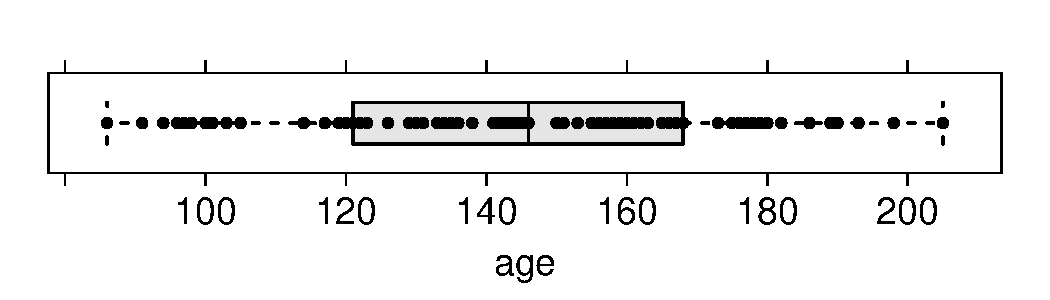
\includegraphics[width=1\textwidth]{/media/data/dyslexia_project/plot/bw_age.pdf}
% \caption{Age distribution.}
% \label{fig:1}
% \end{figure}

% \textbf{Clinical profile:}\\
% \begin{itemize}
% \item DSM5: classification of dyslexia in `low' (class 1), `medium'
%   (class 2), `high' (class 3).\\

% \begin{table}[h!]
%   \begin{center}
%   \begin{tabular}{|c|c|}
%     \hline
%     DSM5 class & number of subjects\\
%     \hline \hline
%     class 1 & 42\\
%     \hline
%     class 2 & 14\\
%     \hline
%     class 3 & 30\\
%     \hline
%   \end{tabular}
% \caption{Clinical profile. DSM5 classification.}
% \label{tab:1}
% \end{center}
% \end{table}

% \end{itemize}

% \textbf{Cognitivie profile:}\\
% \begin{itemize}
% \item WISC-III/IV: 5 \emph{scores}, 7 \emph{subscales}.\\
%   Only the subscale scores are considered. This in order to perform
%   machine learning procedures without involving dependent variables.\\
%   The subscale scores were reduced to 7 after the two instruments,
%   WISC-III and WISC-IV, were merged.

%   Subscale mean: $10$.\\
%   Subscale standard deviation: $3$.
% \begin{table}[h!]
% \begin{center}
%   \begin{tabular}{|c|c|c|c|}
%     \hline
%     WISC subscales & range & mean & sd\\
%     \hline \hline
%     dc & $6:18$&$11.13$&$2.86$\\
%     \hline
%     so & $4:17$&$10.36$&$2.79$\\
%     \hline
%     mc & $2:15$&$8.40$&$2.75$\\
%     \hline
%     cf & $1:14$&$7.60$&$2.67$\\
%     \hline
%     vc & $3:17$&$10.02$&$2.73$\\
%     \hline
%     co & $5:19$&$11.08$&$2.70$\\
%     \hline
%     rs & $2:16$&$9.36$&$2.88$\\
%     \hline
%   \end{tabular}
% \end{center}
% \caption{Cognitive profile. WISC subscales.}
% \label{tab:2}
% \end{table}

% \begin{figure}[h!] 
% \centering
% 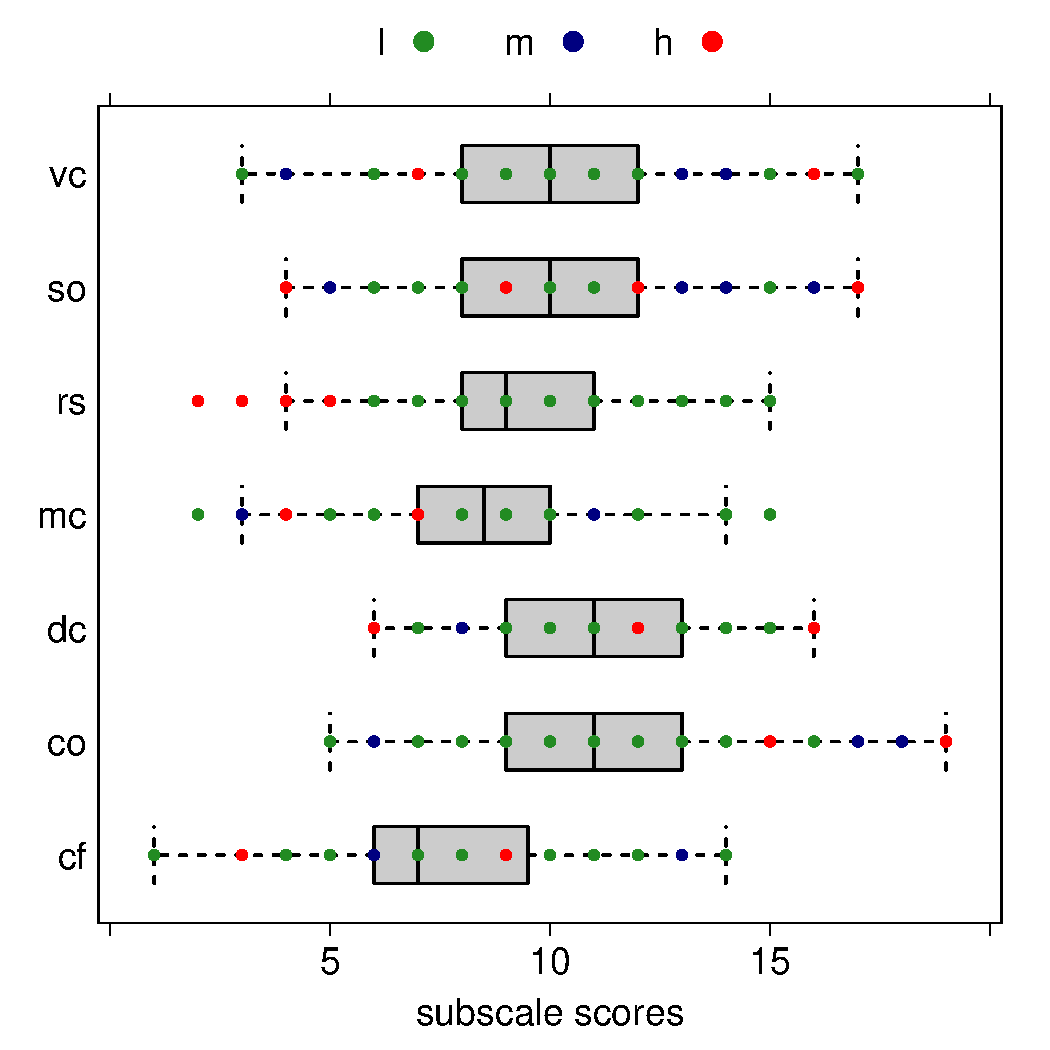
\includegraphics[width=1\textwidth]{/media/data/dyslexia_project/plot/bw_wisc_no_out.pdf}
% \caption{WISC subscale distribution.}
% \label{fig:2}
% \end{figure}

% \begin{figure}[h!] 
% \centering
% 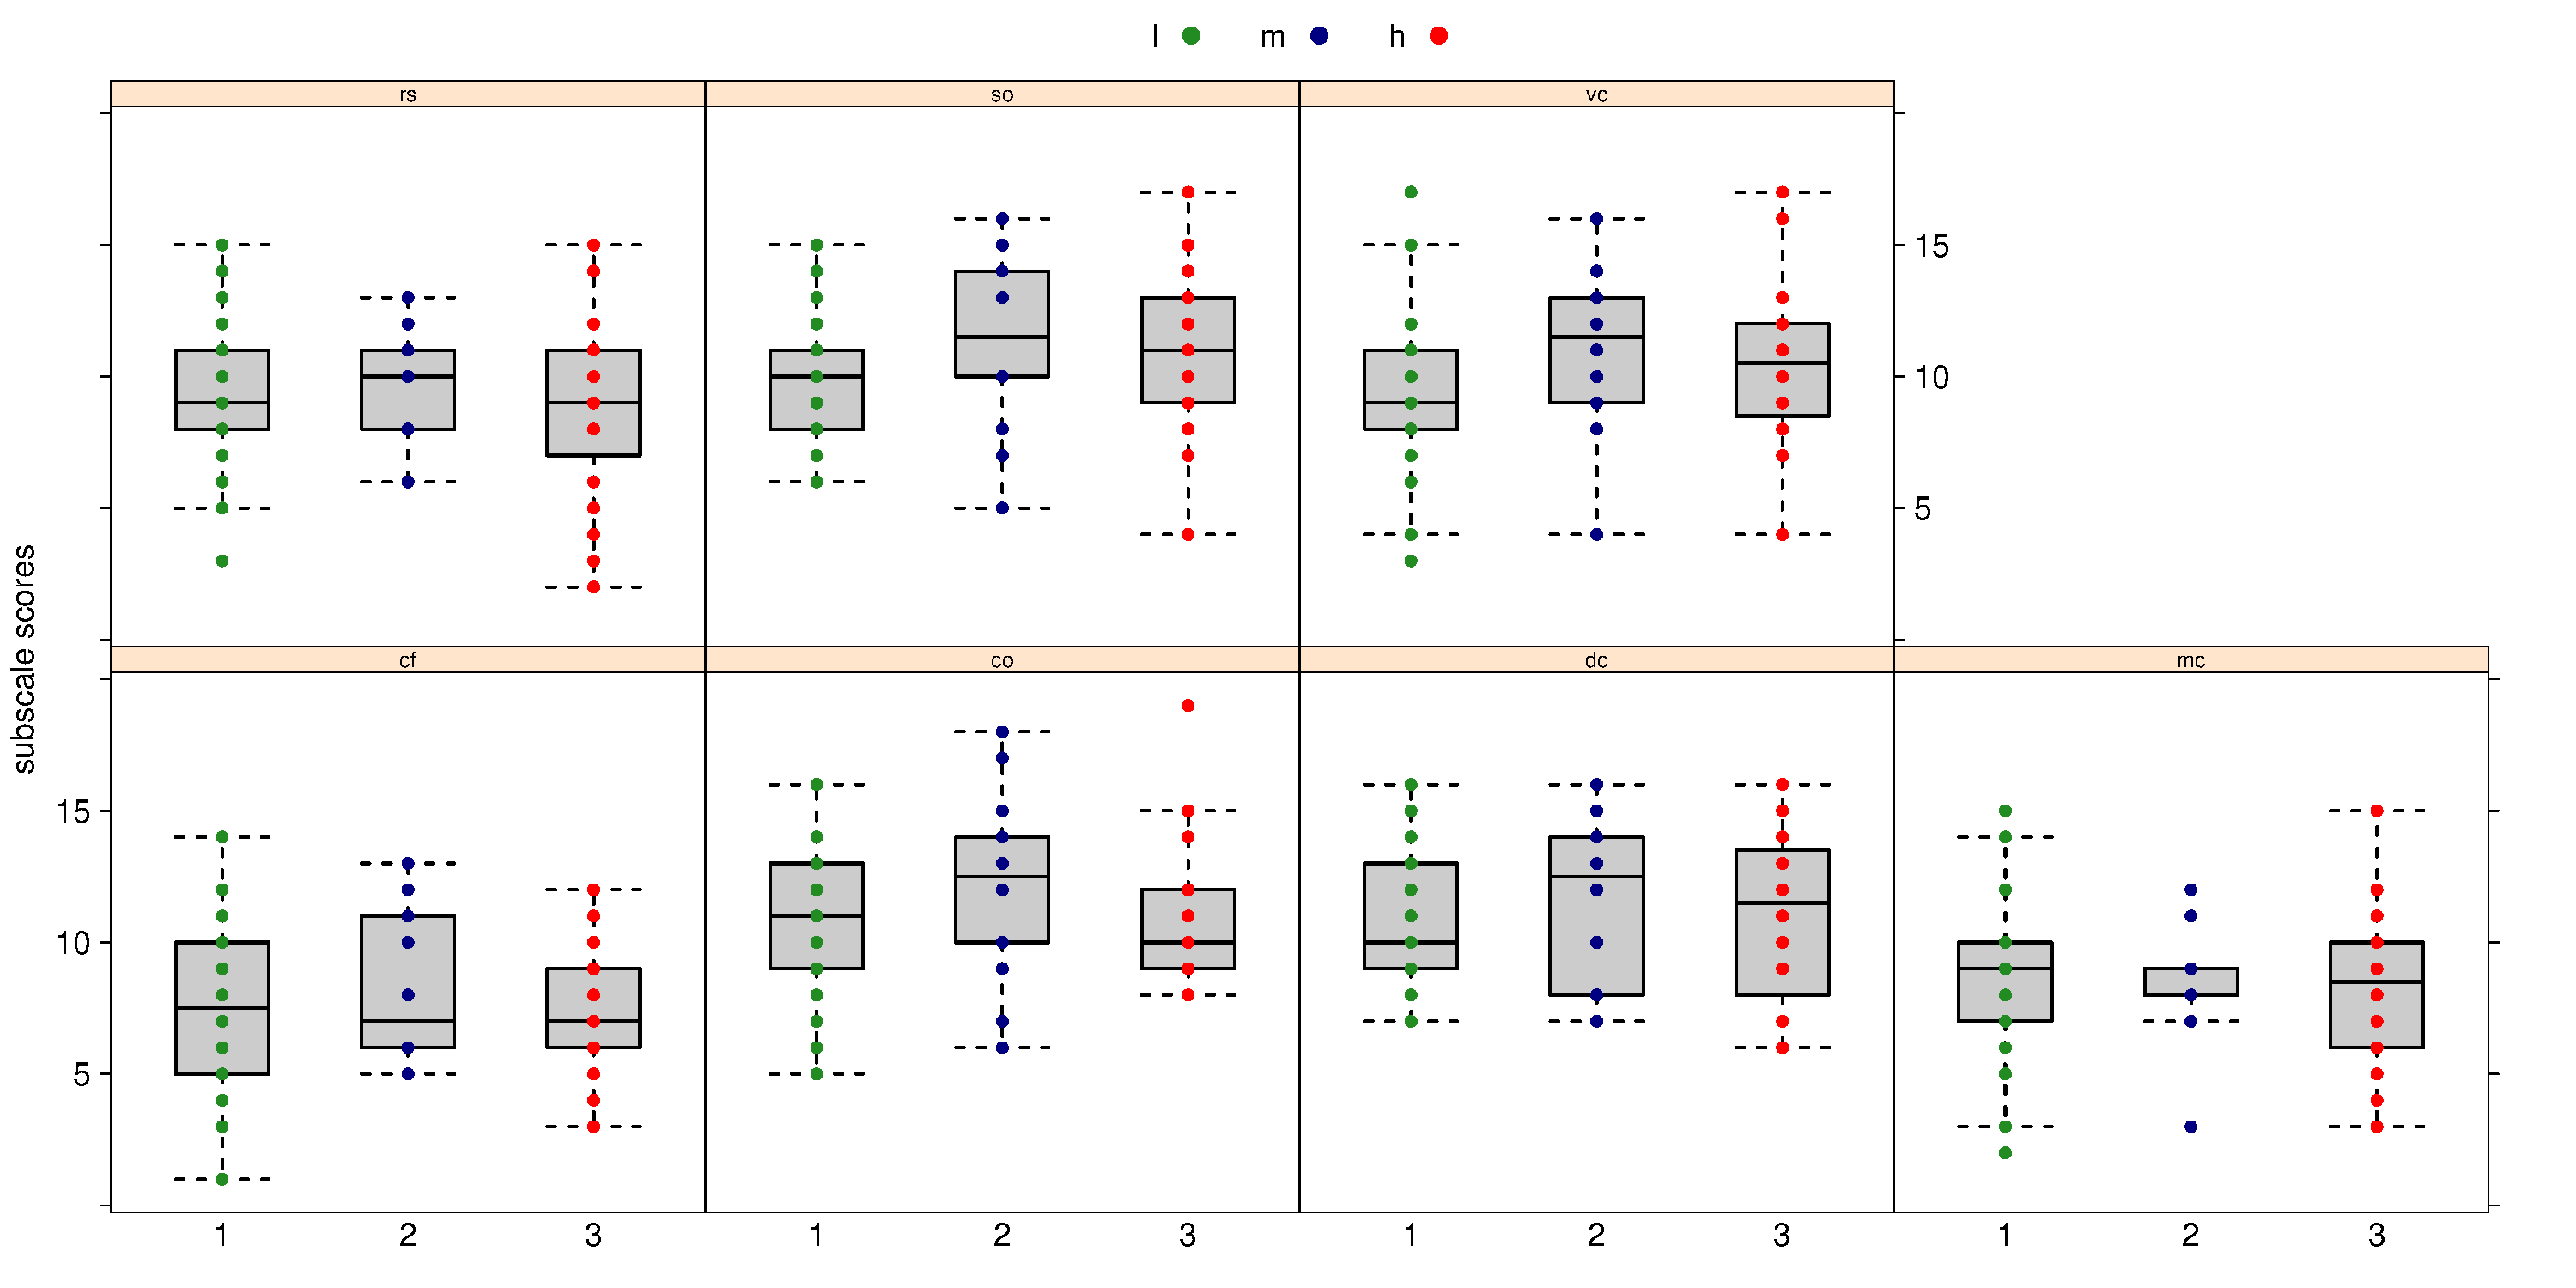
\includegraphics[width=1\textwidth]{/media/data/dyslexia_project/plot/bw_wisc_no_out_class.pdf}
% \caption{WISC subscale distribution by class.}
% \label{fig:3}
% \end{figure}

% \clearpage

% \item DDE: 4 \emph{scores} measuring word/non-word reading speed
%   (wspeed, nwspeed) and accuracy (wacc, nwacc).\\
%   DDE scores are sigma values, with $-2.0$ as the threshold for
%   impairment. These values are computed with respect to age.
% \begin{table}[h!]
% \begin{center}
%   \begin{tabular}{|c|c|c|c|}
%     \hline
%     DDE scores & range & mean & sd\\
%     \hline \hline
%     wspeed & $-13.43:-0.46$ & $-3.93$ & $2.61$\\
%     \hline
%     wacc & $-10.30:1.00$ & $-2.50$ & $2.40$\\
%     \hline
%     nwspeed & $-9.90:0.20$ & $-3.57$ & $2.24$\\
%     \hline
%     nwacc & $-9.00:1.30$ & $-1.33$ & $1.74$\\
%     \hline
%   \end{tabular}
% \end{center}
% \caption{Cognitive profile. DDE scores.}
% \label{tab:3}
% \end{table}

% Outliers: subject 5, 673.\\
% Subject 5 $\longrightarrow$ wspeed$=-13.43$, new range $-11.60:-0.46$\\
% Subject 673 $\longrightarrow$ nwacc$=-9.00$, new range $-4.40:1.30$

% \begin{figure}[h!] 
% \centering
% 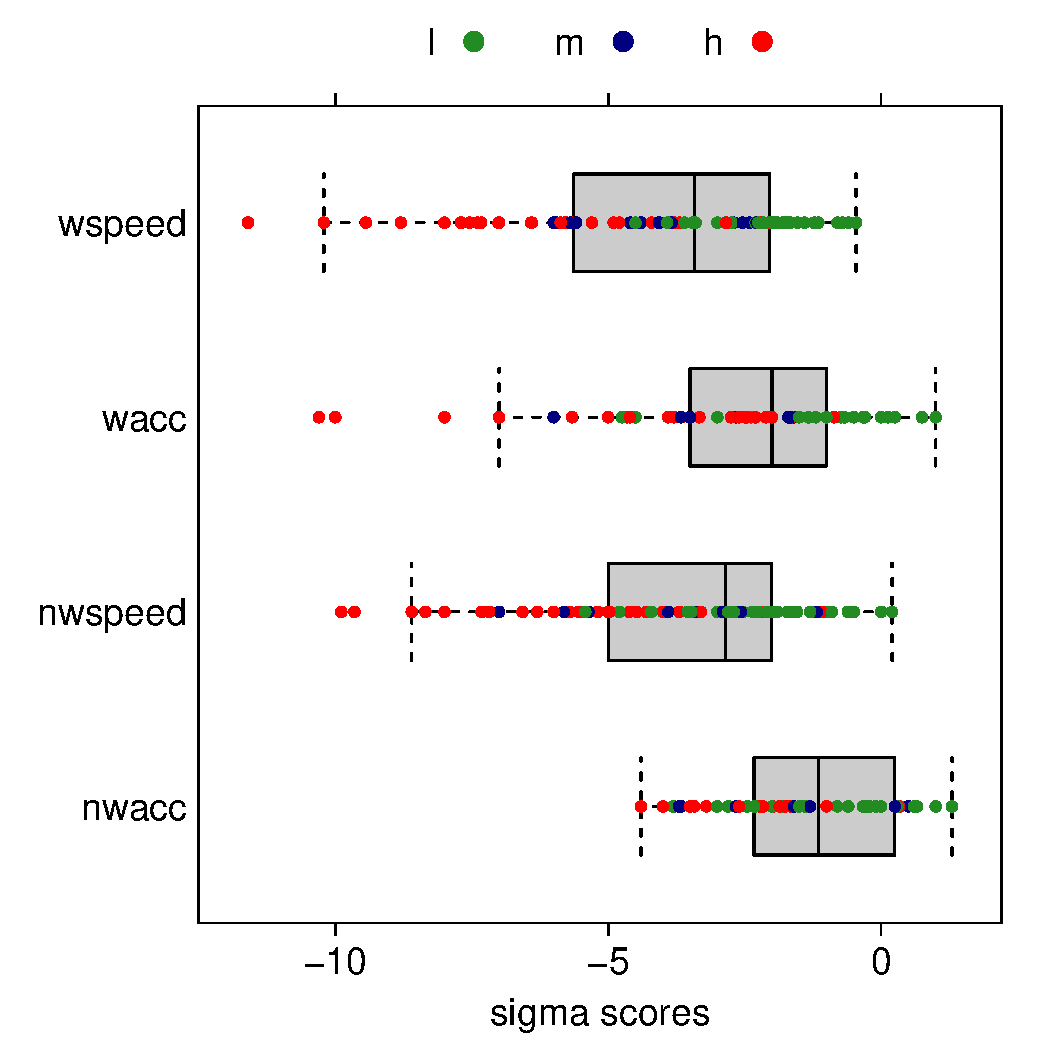
\includegraphics[width=1\textwidth]{/media/data/dyslexia_project/plot/bw_dde_no_out.pdf}
% \caption{DDE score distribution.}
% \label{fig:4}
% \end{figure}

% % \begin{figure}[h!] 
% % \centering
% % 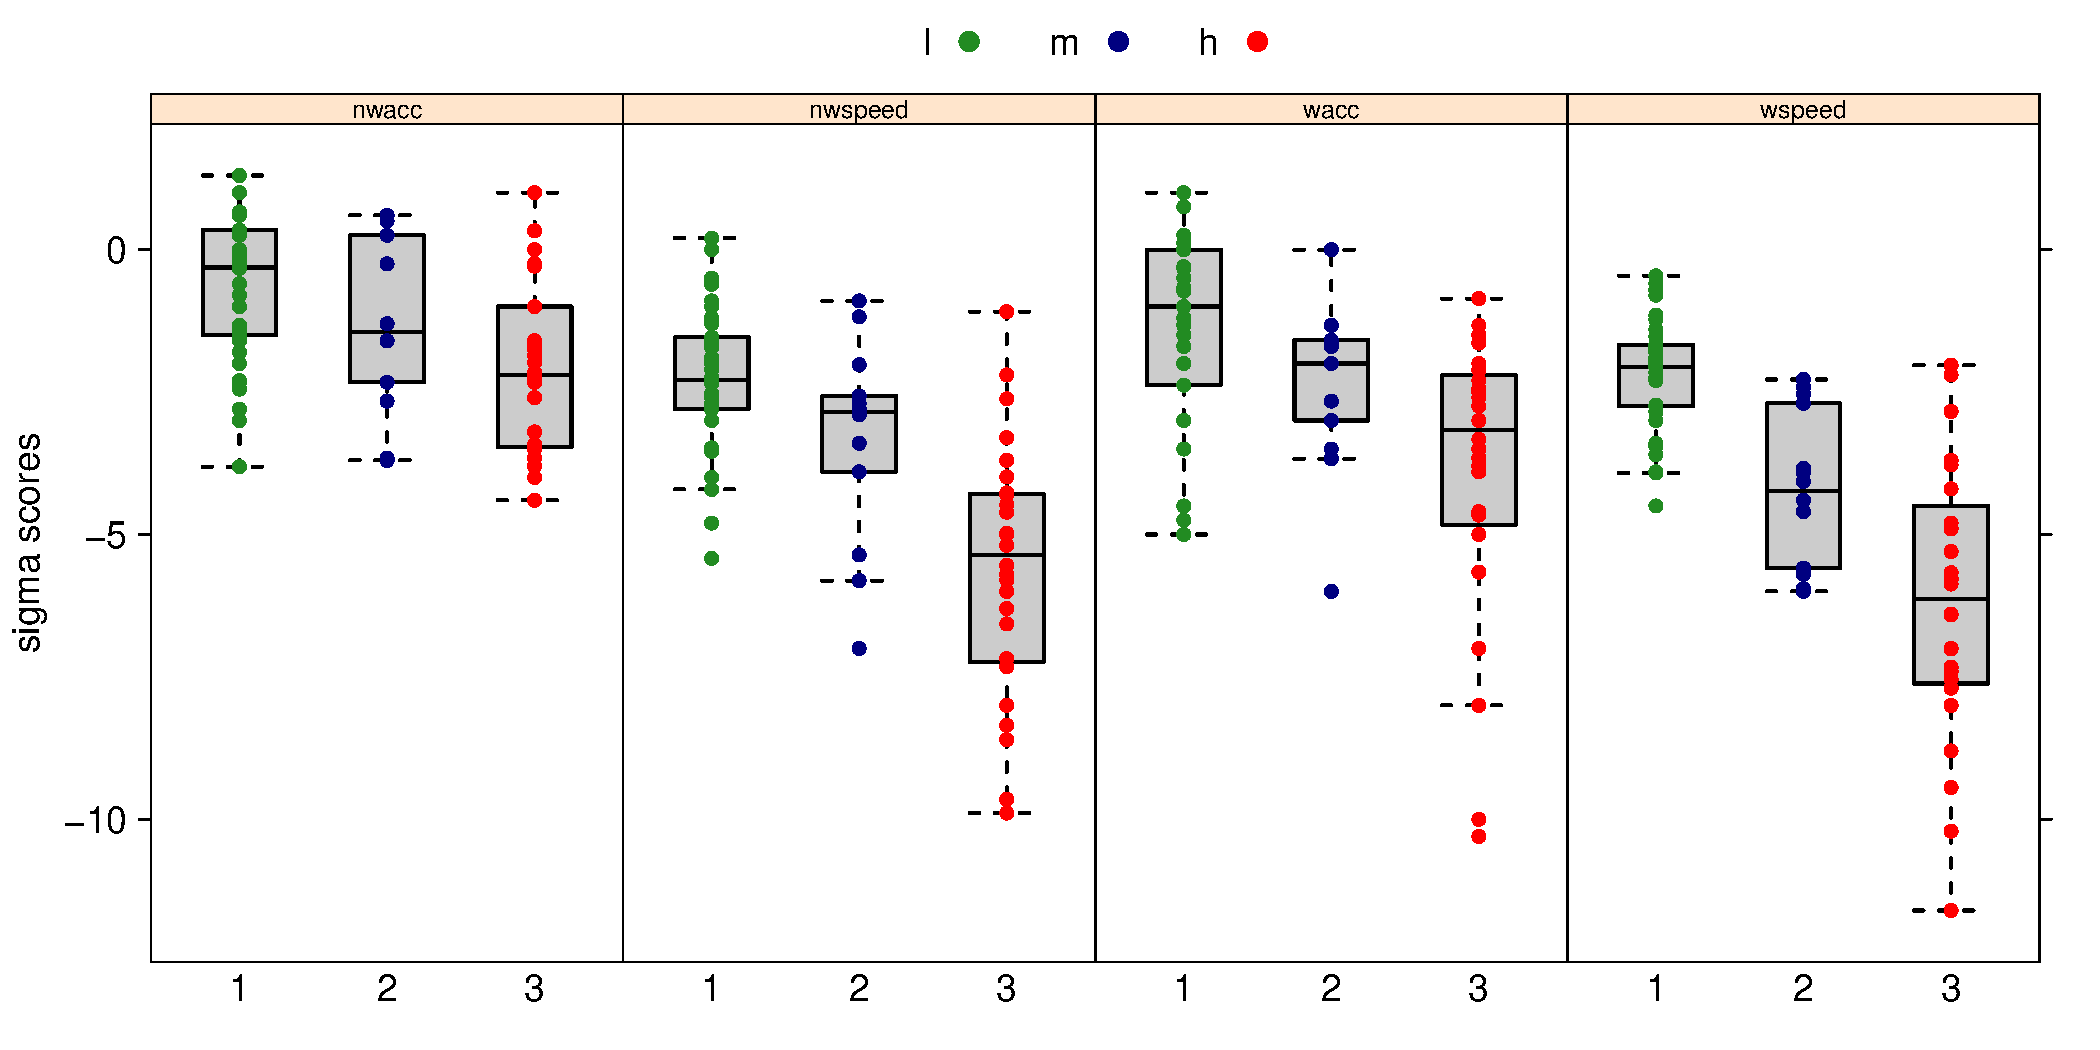
\includegraphics[width=1\textwidth]{/media/data/dyslexia_project/plot/bw_dde_no_out_class.pdf}
% % \caption{DDE score distribution by class.}
% % \label{fig:5}
% % \end{figure}

% \end{itemize}

% \clearpage

% In order to investigate the distribution of DSM5 classes and the
% correlation between the scores we provide the graph below.
% \begin{figure}[h!] 
% \centering
% 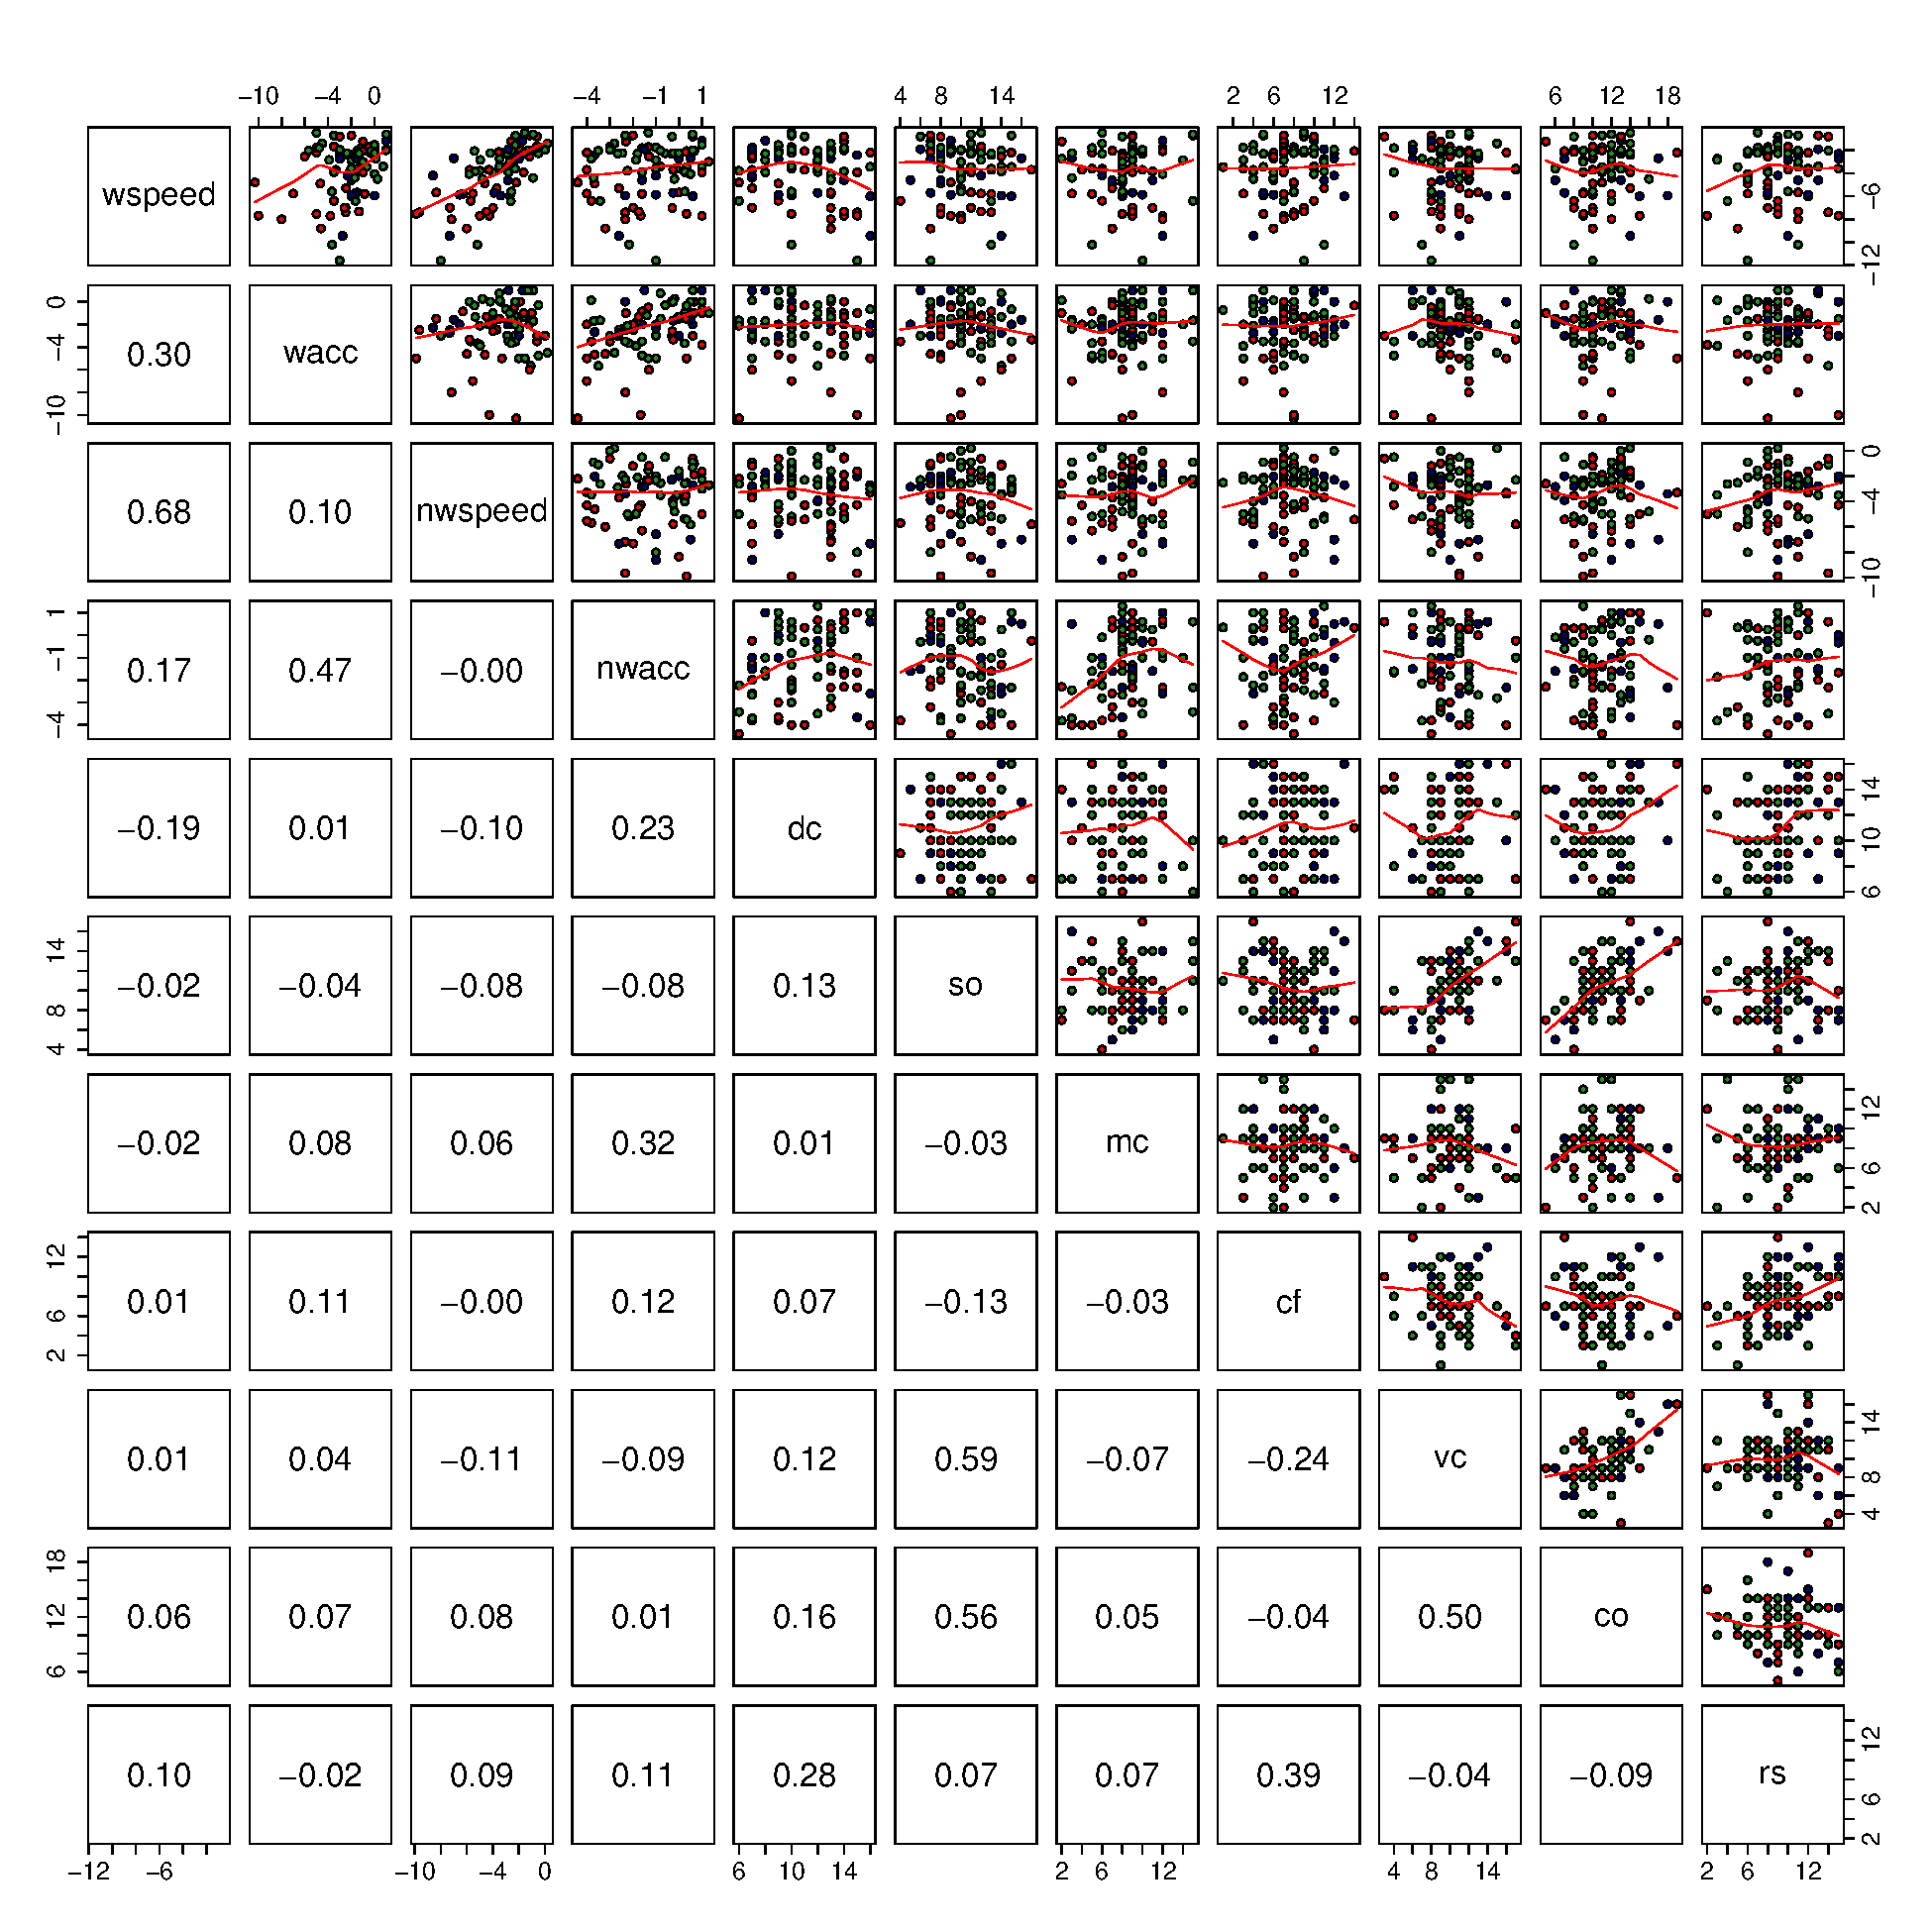
\includegraphics[width=1\textwidth]{/media/data/dyslexia_project/plot/pairs_no_out.pdf}
% \caption{Pair graph with DDE scores and WISC subscales. Correlation coefficient in the lower panel.}
% \label{fig:6}
% \end{figure}

% \clearpage

% \section{Visual Data Analysis}
% From previous Figures we can suppose that DSM5 classification can be
% driven from DDE scores, hence DDE is a classifier, while WISC
% subscales work as a modulator. We want to assess the following diagram
% in order to provide a cognitive profile to the DSM5 classification (*).

% \begin{center}
% \begin{tikzpicture}
%   \matrix (m) [matrix of math nodes,row sep=3em,column sep=4em,minimum width=2em]
%   {
%      DY_T\ (DDE) & DY_C\ (DSM5) \\
%      I\ (WISC) & \\};
%   \path[-stealth]
%     (m-2-1) edge node [left] {} (m-1-1)
%     (m-1-1) edge [left] node [below] {} (m-1-2)
%     (m-2-1) edge [dashed] node [below] {*} (m-1-2);
% \end{tikzpicture}
% \end{center}

% \small{$DY_T$: technical dyslexia, $DY_C$: clinical dyslexia, $I$: intelligence.}

% \subsection{DDE scores}
% Firstly we want to see if it is possible to reduce the number of DDE
% variables, from 4 to 2, expressing the processing speed in function of
% the processing accuracy.
% \begin{figure}[h!] 
% \centering 
% \begin{subfigure}{1\textwidth}
% \centering
% 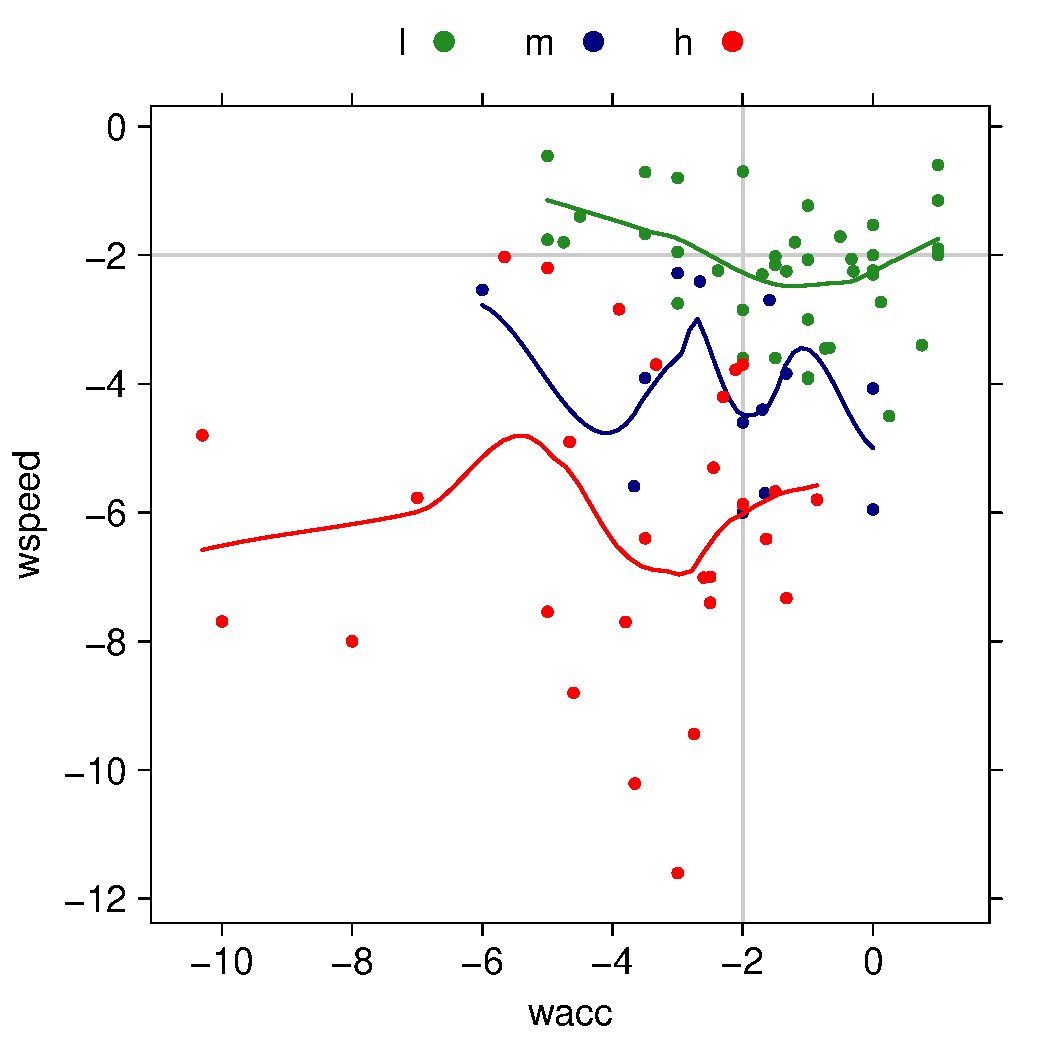
\includegraphics[width=1\textwidth]{/media/data/dyslexia_project/plot/scat_ddew_no_out.pdf}
% \caption{Scatterplot word accuracy against word speed in the three classes.}
% \label{fig:7a}
% \end{subfigure}
% \end{figure}
% \begin{figure}
% \ContinuedFloat
% \centering 
% \begin{subfigure}{1\textwidth}
% \centering
% 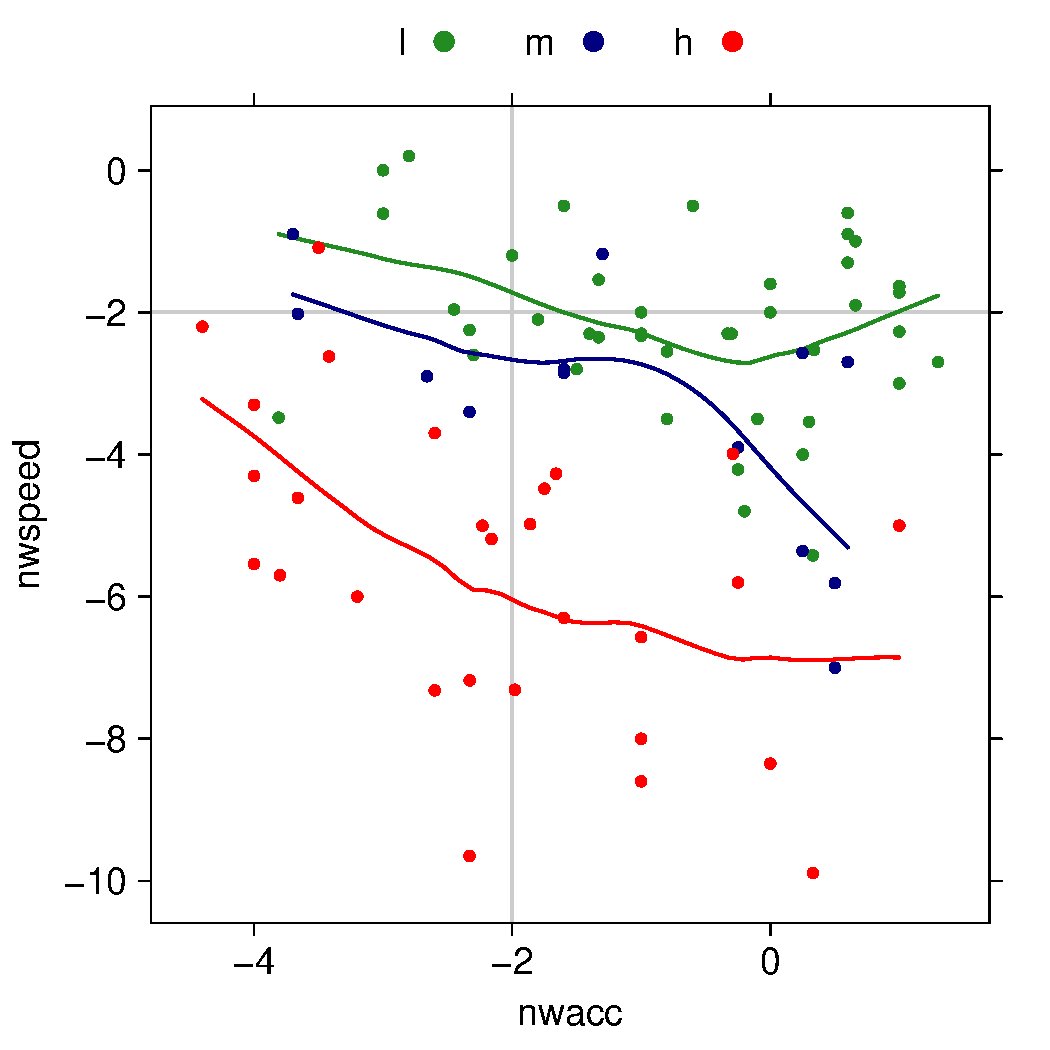
\includegraphics[width=1\textwidth]{/media/data/dyslexia_project/plot/scat_ddenw_no_out.pdf}
% \caption{Scatterplot non-word accuracy against non-word speed in the three classes.}
% \label{fig:7b}
% \end{subfigure}
% \caption{}
% \label{fig:7}
% \end{figure}

% \clearpage

% \subsection{WISC subscales}
% We would like to parametrize the loess lines in
% Figures~\ref{fig:7a}-\ref{fig:7b} in order to see if the variation of
% WISC subscales determines a shift from the curve of one class to the
% curve of another.\\
% Let us now see how the WISC subscales vary according to the DDE
% word/non-word speed scores. We highlight the first and third quantile,
% along with the DSM5 classes.

% \begin{figure}[h!] 
% \centering 
% \begin{subfigure}{1\textwidth}
% \centering
% 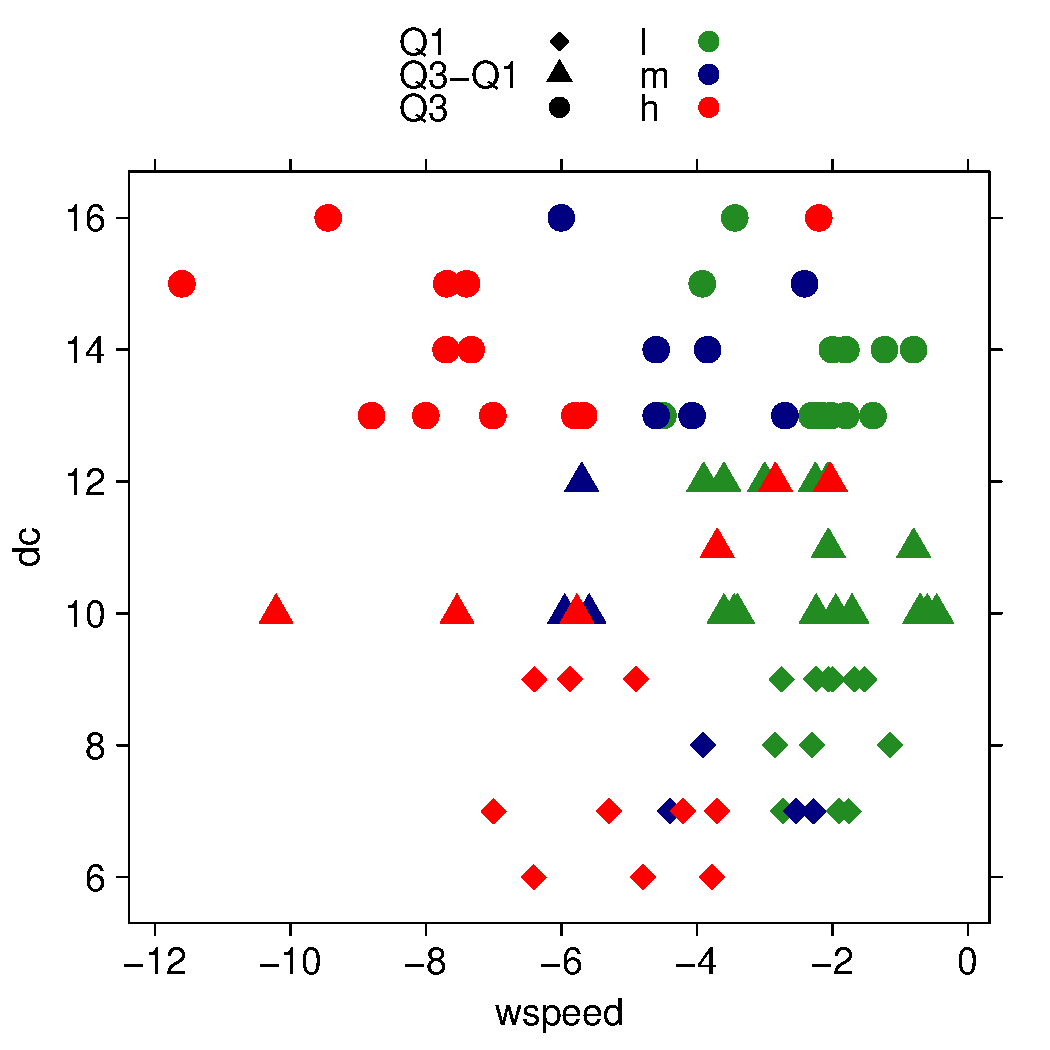
\includegraphics[width=1\textwidth]{/media/data/dyslexia_project/plot/ws_dc.pdf}
% \caption{}
% \label{fig:8a}
% \end{subfigure}
% \end{figure}
% \begin{figure}
% \ContinuedFloat
% \centering 
% \begin{subfigure}{1\textwidth}
% \centering
% 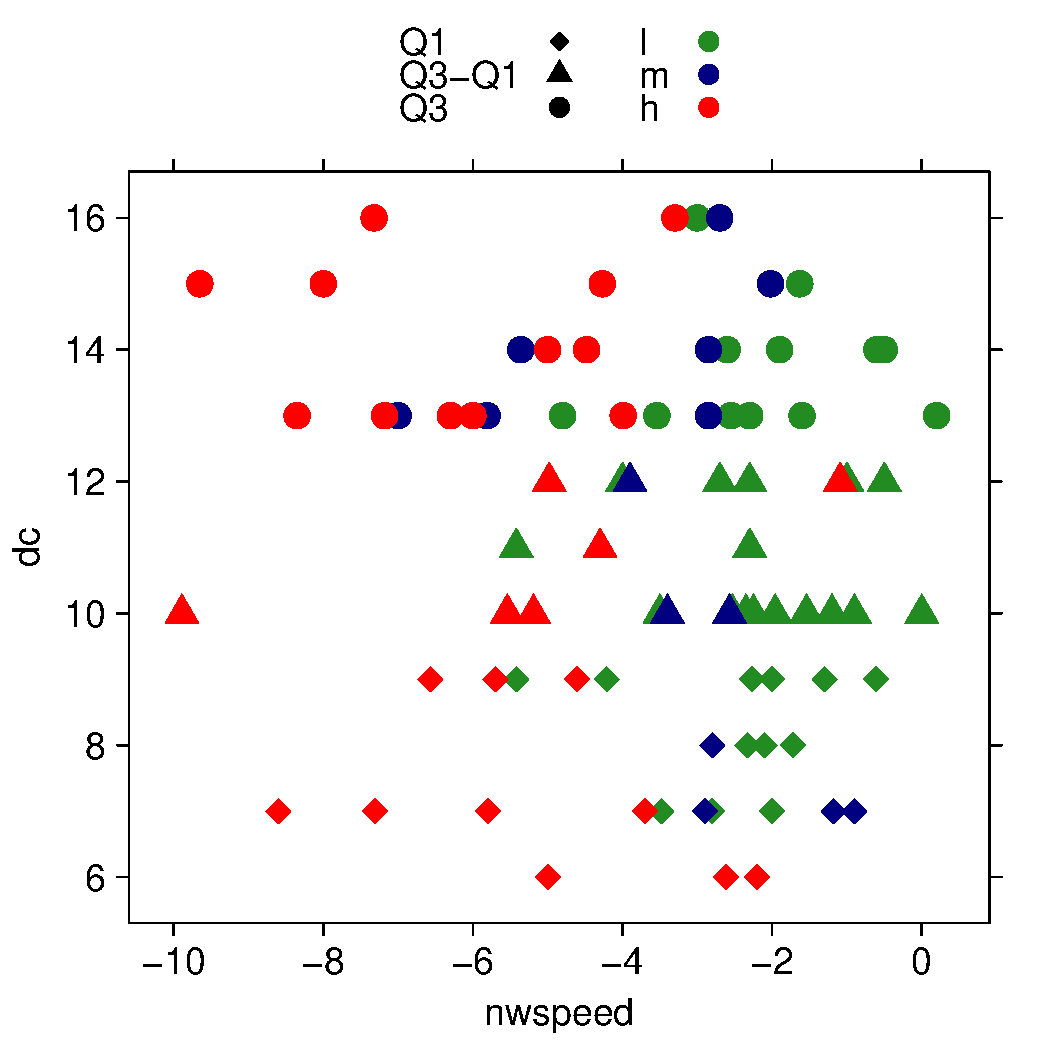
\includegraphics[width=1\textwidth]{/media/data/dyslexia_project/plot/nws_dc.pdf}
% \caption{}
% \label{fig:8b}
% \end{subfigure}
% \caption{Reading speed of words and non-words against subscale dc.}
% \label{fig:8}
% \end{figure}

% \begin{figure}[h!] 
% \centering 
% \begin{subfigure}{1\textwidth}
% \centering
% 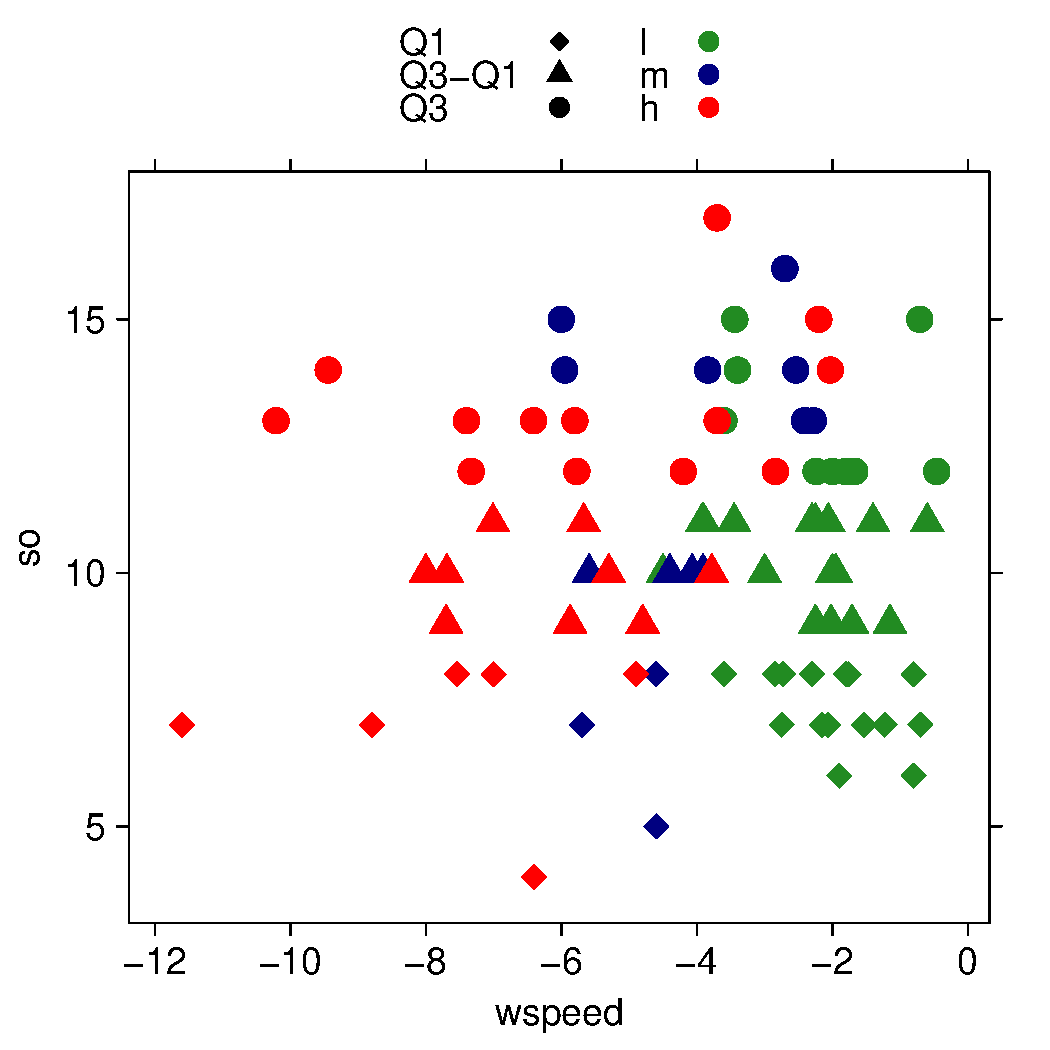
\includegraphics[width=1\textwidth]{/media/data/dyslexia_project/plot/ws_so.pdf}
% \caption{}
% \label{fig:9a}
% \end{subfigure}
% \end{figure}
% \begin{figure}
% \ContinuedFloat
% \centering 
% \begin{subfigure}{1\textwidth}
% \centering
% 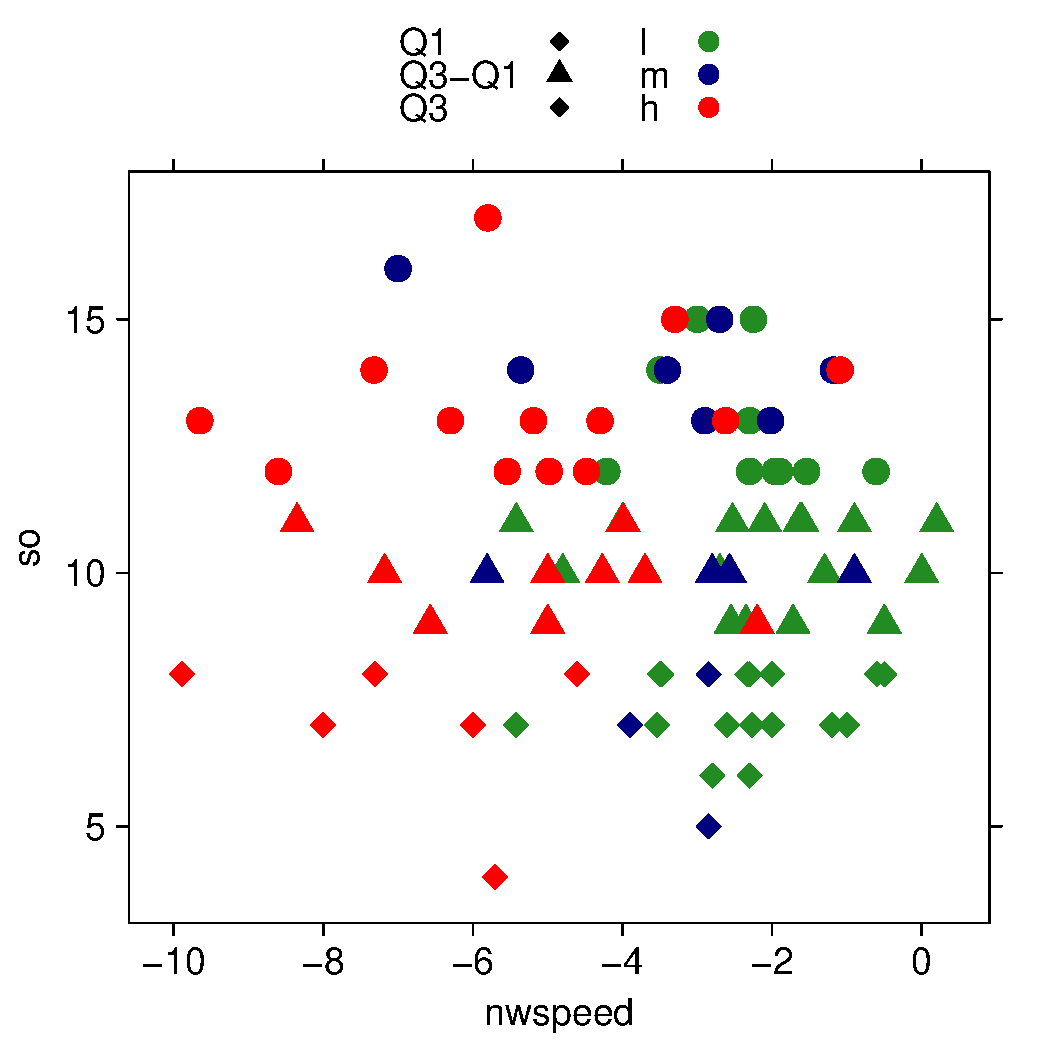
\includegraphics[width=1\textwidth]{/media/data/dyslexia_project/plot/nws_so.pdf}
% \caption{}
% \label{fig:9b}
% \end{subfigure}
% \caption{Reading speed of words and non-words against subscale so.}
% \label{fig:9}
% \end{figure}

% \begin{figure}[h!] 
% \centering 
% \begin{subfigure}{1\textwidth}
% \centering
% 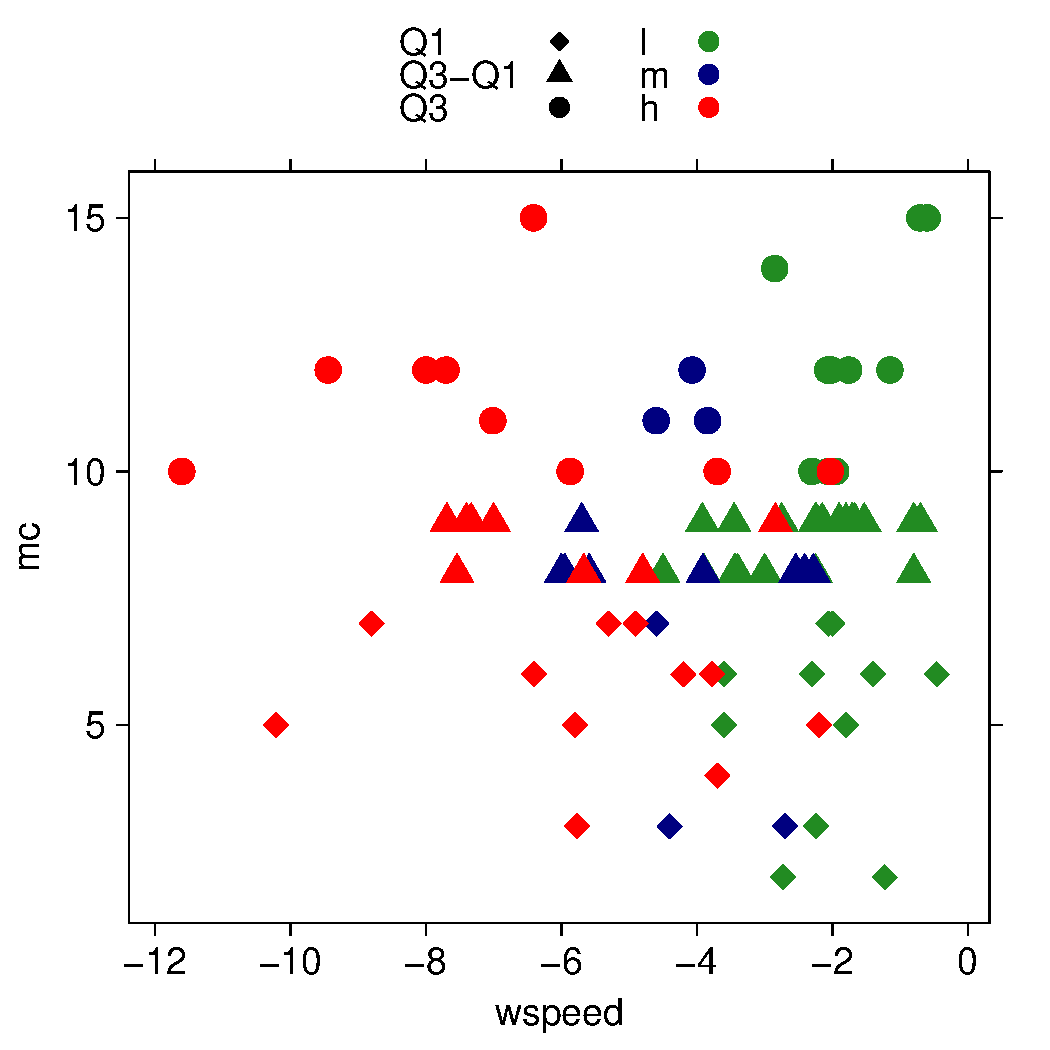
\includegraphics[width=1\textwidth]{/media/data/dyslexia_project/plot/ws_mc.pdf}
% \caption{}
% \label{fig:10a}
% \end{subfigure}
% \end{figure}
% \begin{figure}
% \ContinuedFloat
% \centering 
% \begin{subfigure}{1\textwidth}
% \centering
% 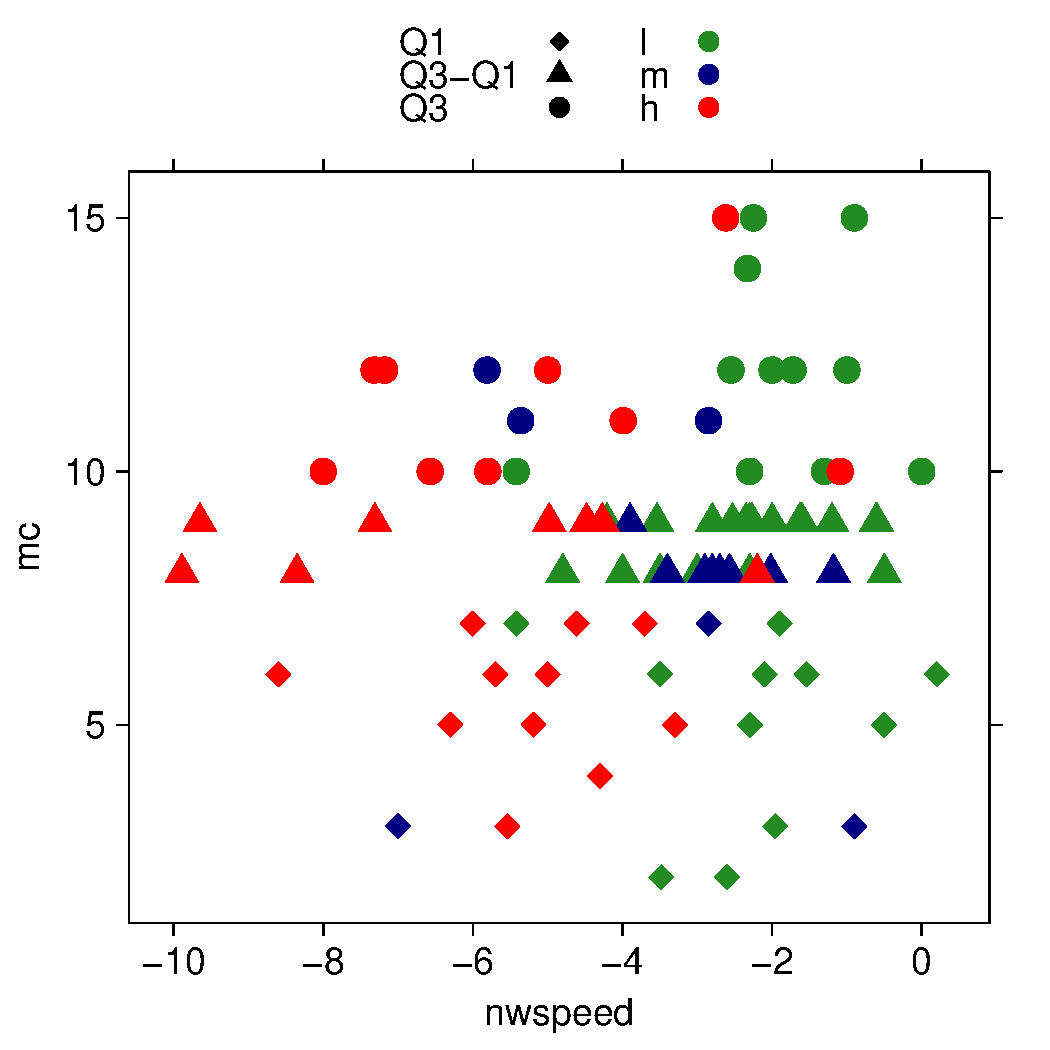
\includegraphics[width=1\textwidth]{/media/data/dyslexia_project/plot/nws_mc.pdf}
% \caption{}
% \label{fig:10b}
% \end{subfigure}
% \caption{Reading speed of words and non-words against subscale mc.}
% \label{fig:10}
% \end{figure}

% \begin{figure}[h!] 
% \centering 
% \begin{subfigure}{1\textwidth}
% \centering
% 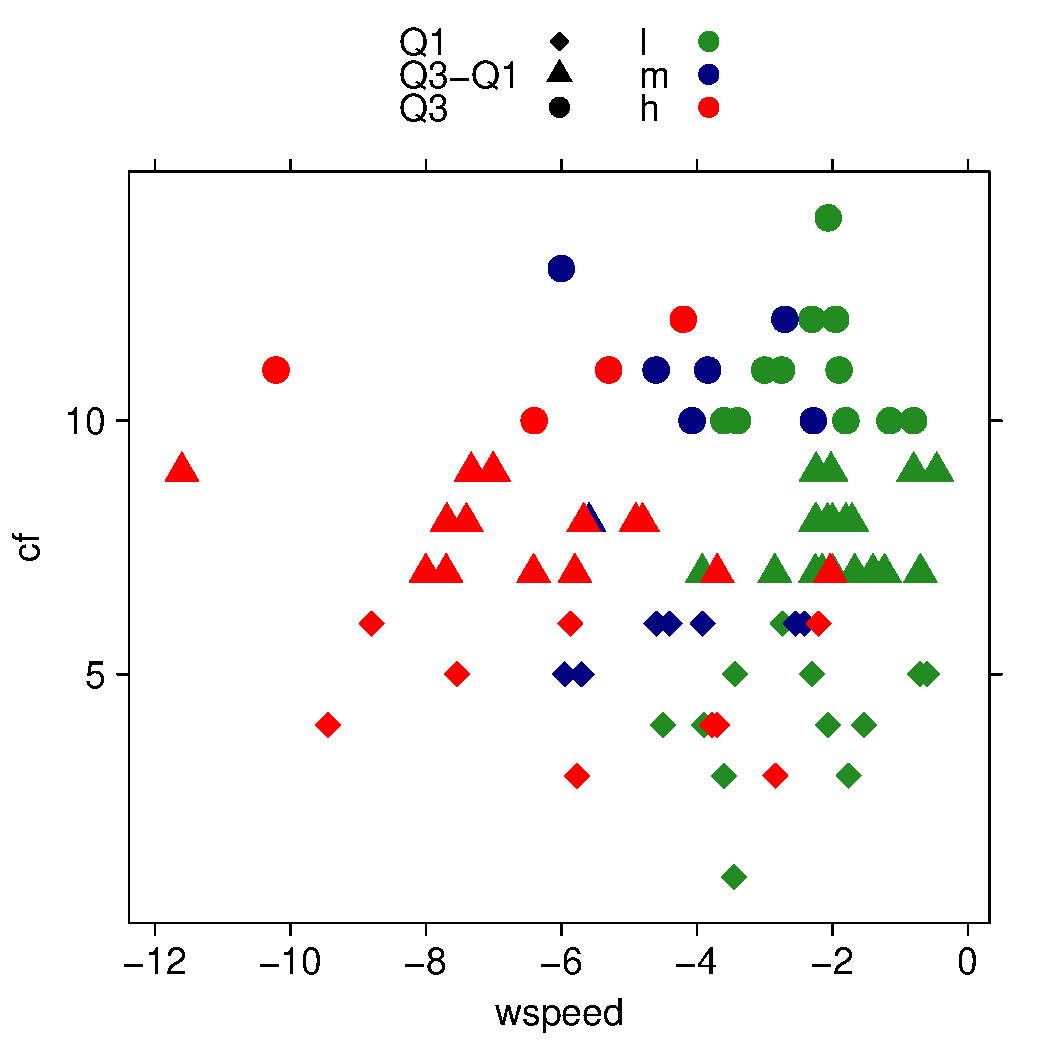
\includegraphics[width=1\textwidth]{/media/data/dyslexia_project/plot/ws_cf.pdf}
% \caption{}
% \label{fig:11a}
% \end{subfigure}
% \end{figure}
% \begin{figure}
% \ContinuedFloat
% \centering 
% \begin{subfigure}{1\textwidth}
% \centering
% 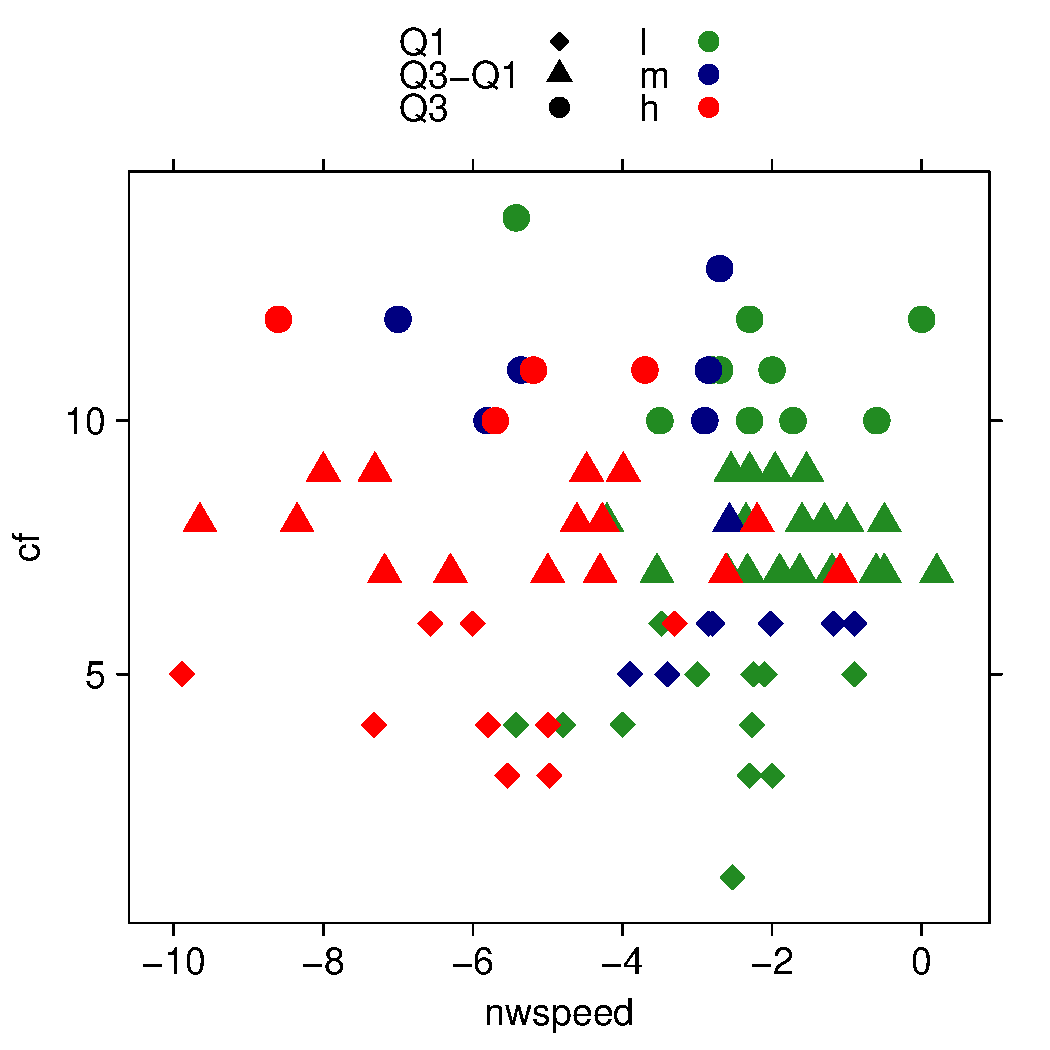
\includegraphics[width=1\textwidth]{/media/data/dyslexia_project/plot/nws_cf.pdf}
% \caption{}
% \label{fig:11b}
% \end{subfigure}
% \caption{Reading speed of words and non-words against subscale cf.}
% \label{fig:11}
% \end{figure}

% \begin{figure}[h!] 
% \centering 
% \begin{subfigure}{1\textwidth}
% \centering
% 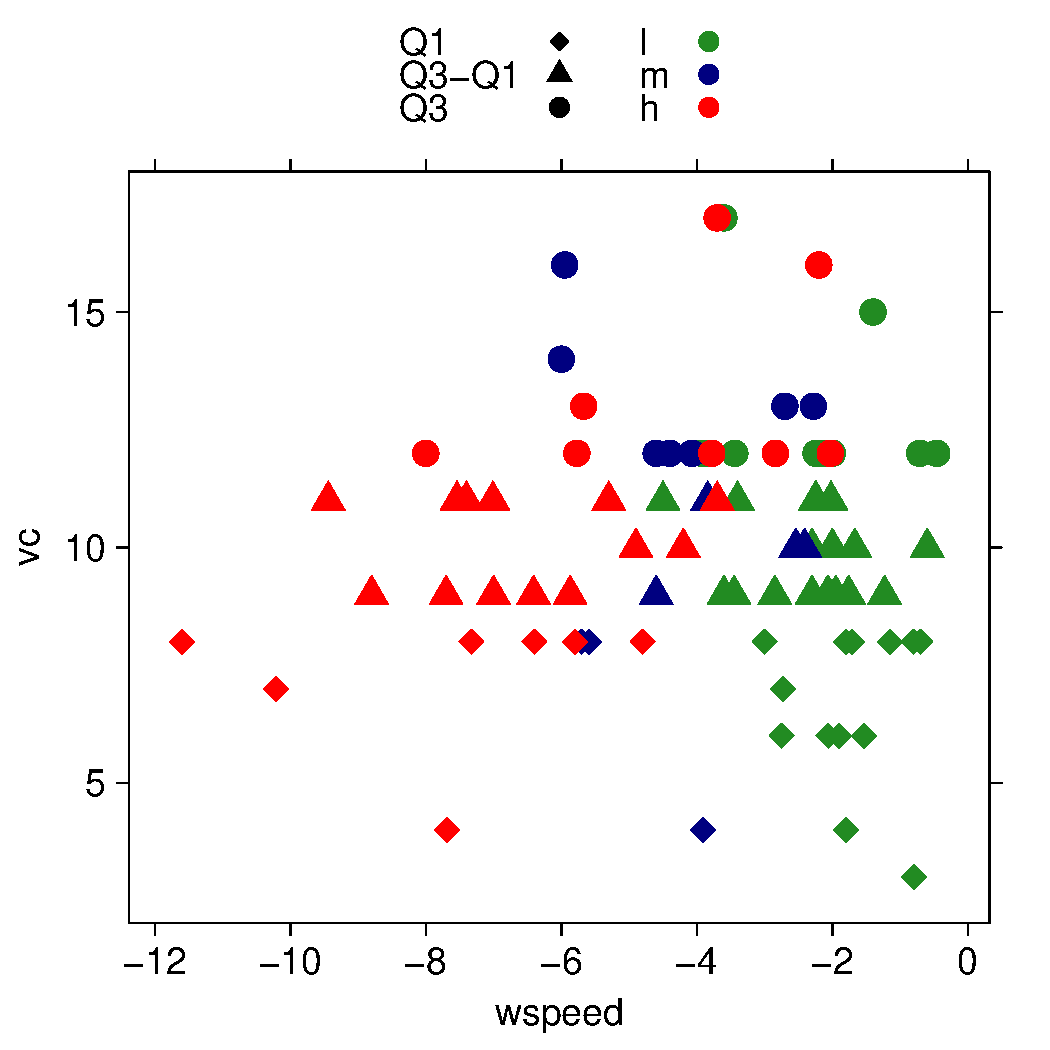
\includegraphics[width=1\textwidth]{/media/data/dyslexia_project/plot/ws_vc.pdf}
% \caption{}
% \label{fig:12a}
% \end{subfigure}
% \end{figure}
% \begin{figure}
% \ContinuedFloat
% \centering 
% \begin{subfigure}{1\textwidth}
% \centering
% 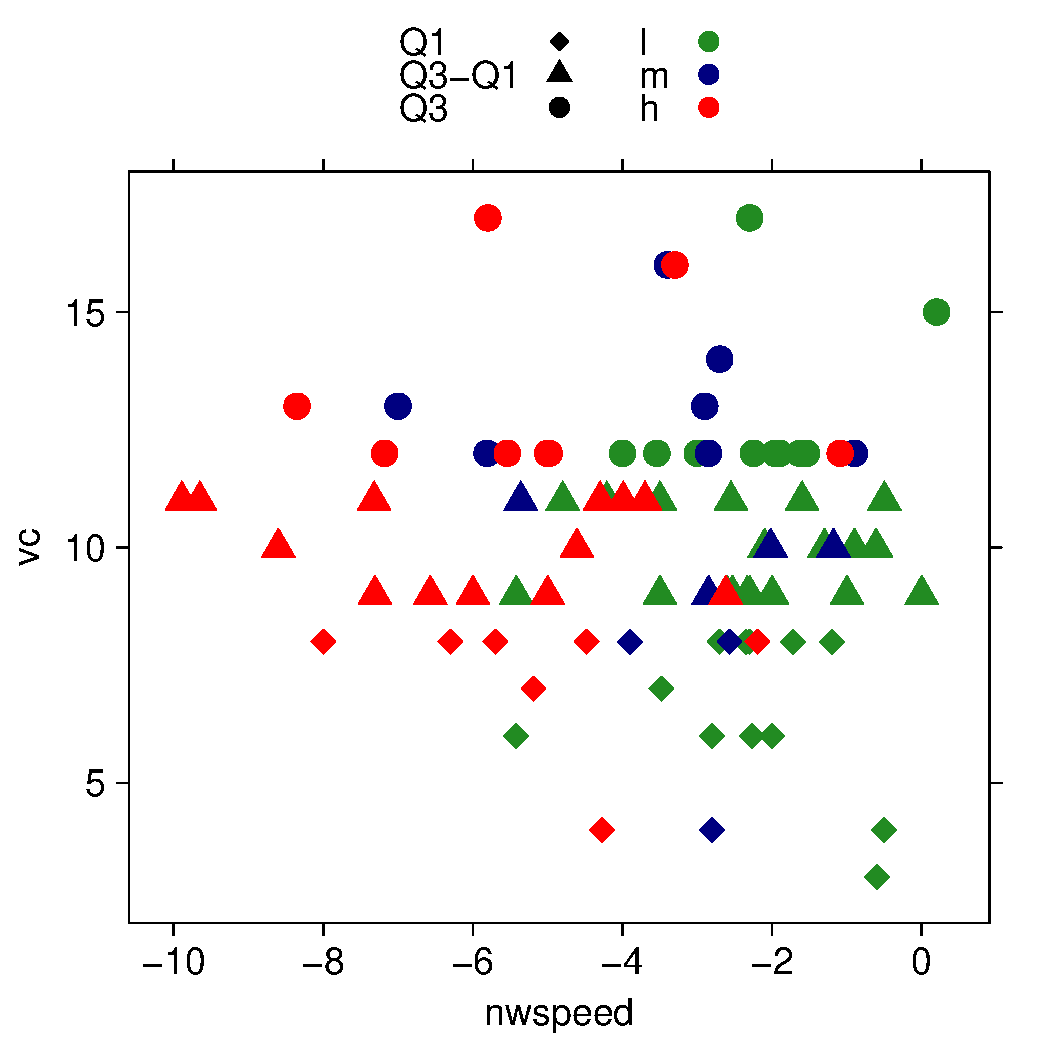
\includegraphics[width=1\textwidth]{/media/data/dyslexia_project/plot/nws_vc.pdf}
% \caption{}
% \label{fig:12b}
% \end{subfigure}
% \caption{Reading speed of words and non-words against subscale vc.}
% \label{fig:12}
% \end{figure}

% \begin{figure}[h!] 
% \centering 
% \begin{subfigure}{1\textwidth}
% \centering
% 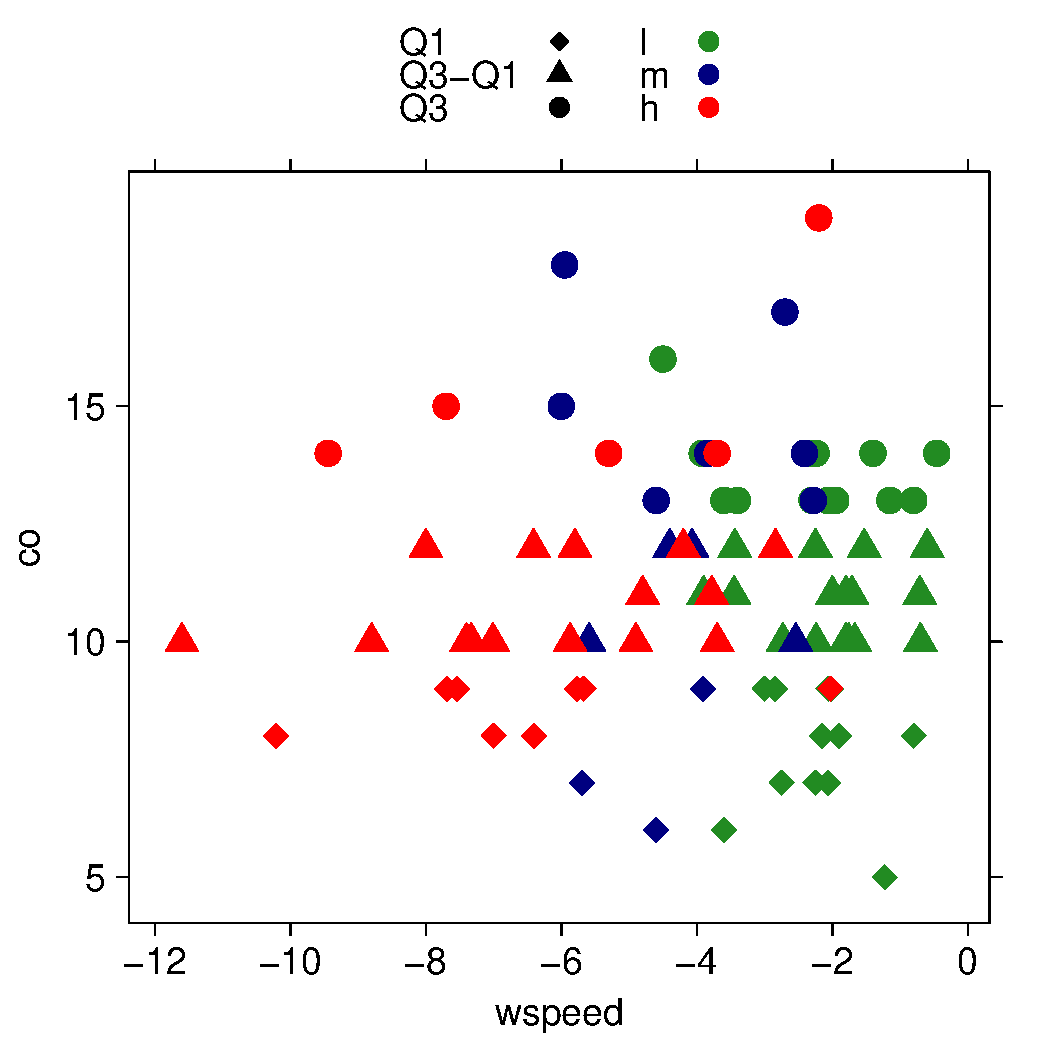
\includegraphics[width=1\textwidth]{/media/data/dyslexia_project/plot/ws_co.pdf}
% \caption{}
% \label{fig:13a}
% \end{subfigure}
% \end{figure}
% \begin{figure}
% \ContinuedFloat
% \centering 
% \begin{subfigure}{1\textwidth}
% \centering
% 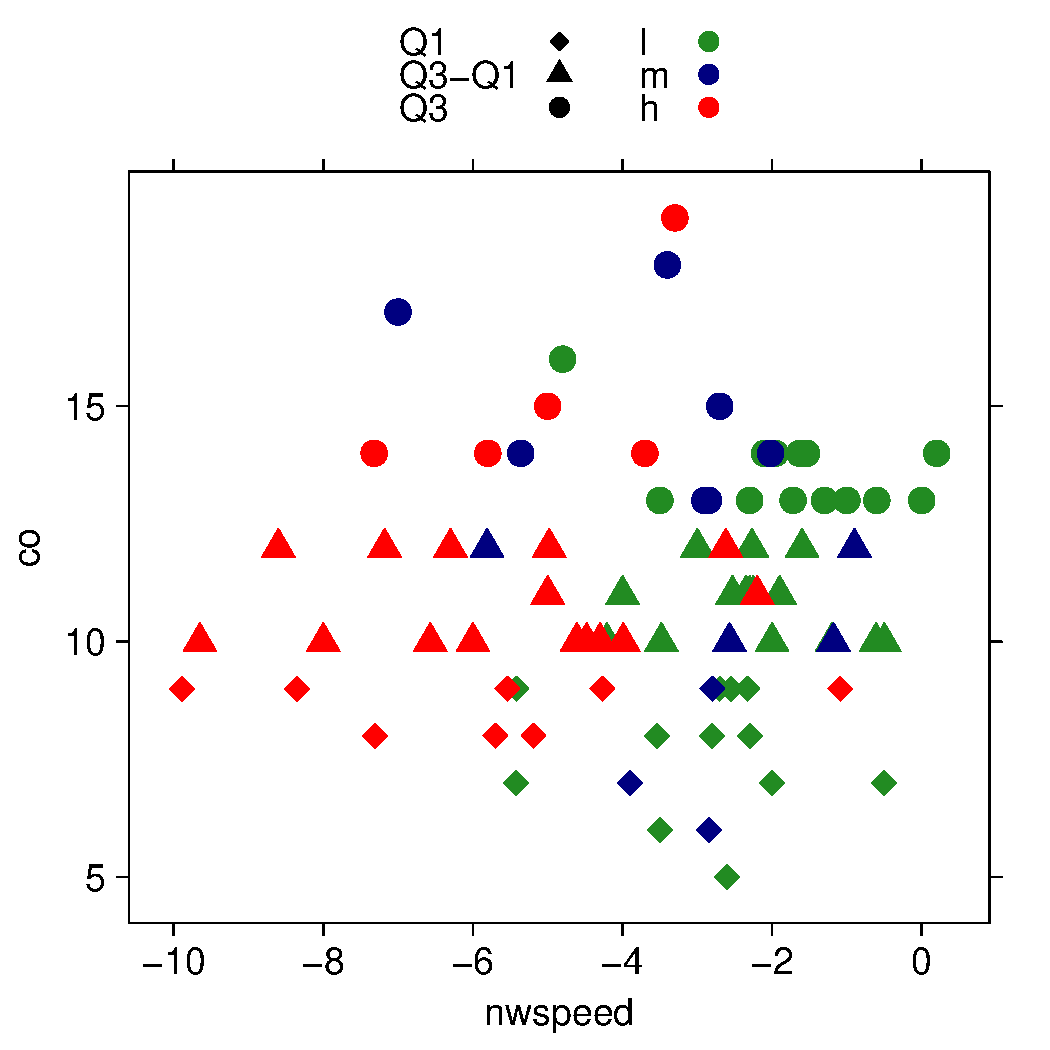
\includegraphics[width=1\textwidth]{/media/data/dyslexia_project/plot/nws_co.pdf}
% \caption{}
% \label{fig:13b}
% \end{subfigure}
% \caption{Reading speed of words and non-words against subscale co.}
% \label{fig:13}
% \end{figure}

% \clearpage

% \section{Data Analysis}
% \subsection{Random Forest}
% Firstly we perform a random forest with classification trees, where we
% try to perform the DSM5 classification with DDE scores.  As we can see
% in Figure~\ref{fig:14} the most important variables are the ones
% concerning the reading speed ability. This supports the thesis that
% dde scores can be reduced from 4 to 2 variables.
% \begin{verbatim}
% Type of random forest: classification
%                      Number of trees: 500
% No. of variables tried at each split: 2

%         OOB estimate of  error rate: 20.93%
% Confusion matrix:
%    1 2  3 class.error
% 1 39 3  0  0.07142857
% 2  6 5  3  0.64285714
% 3  3 3 24  0.20000000
% \end{verbatim}
% \begin{figure}[h!] 
% \centering
% 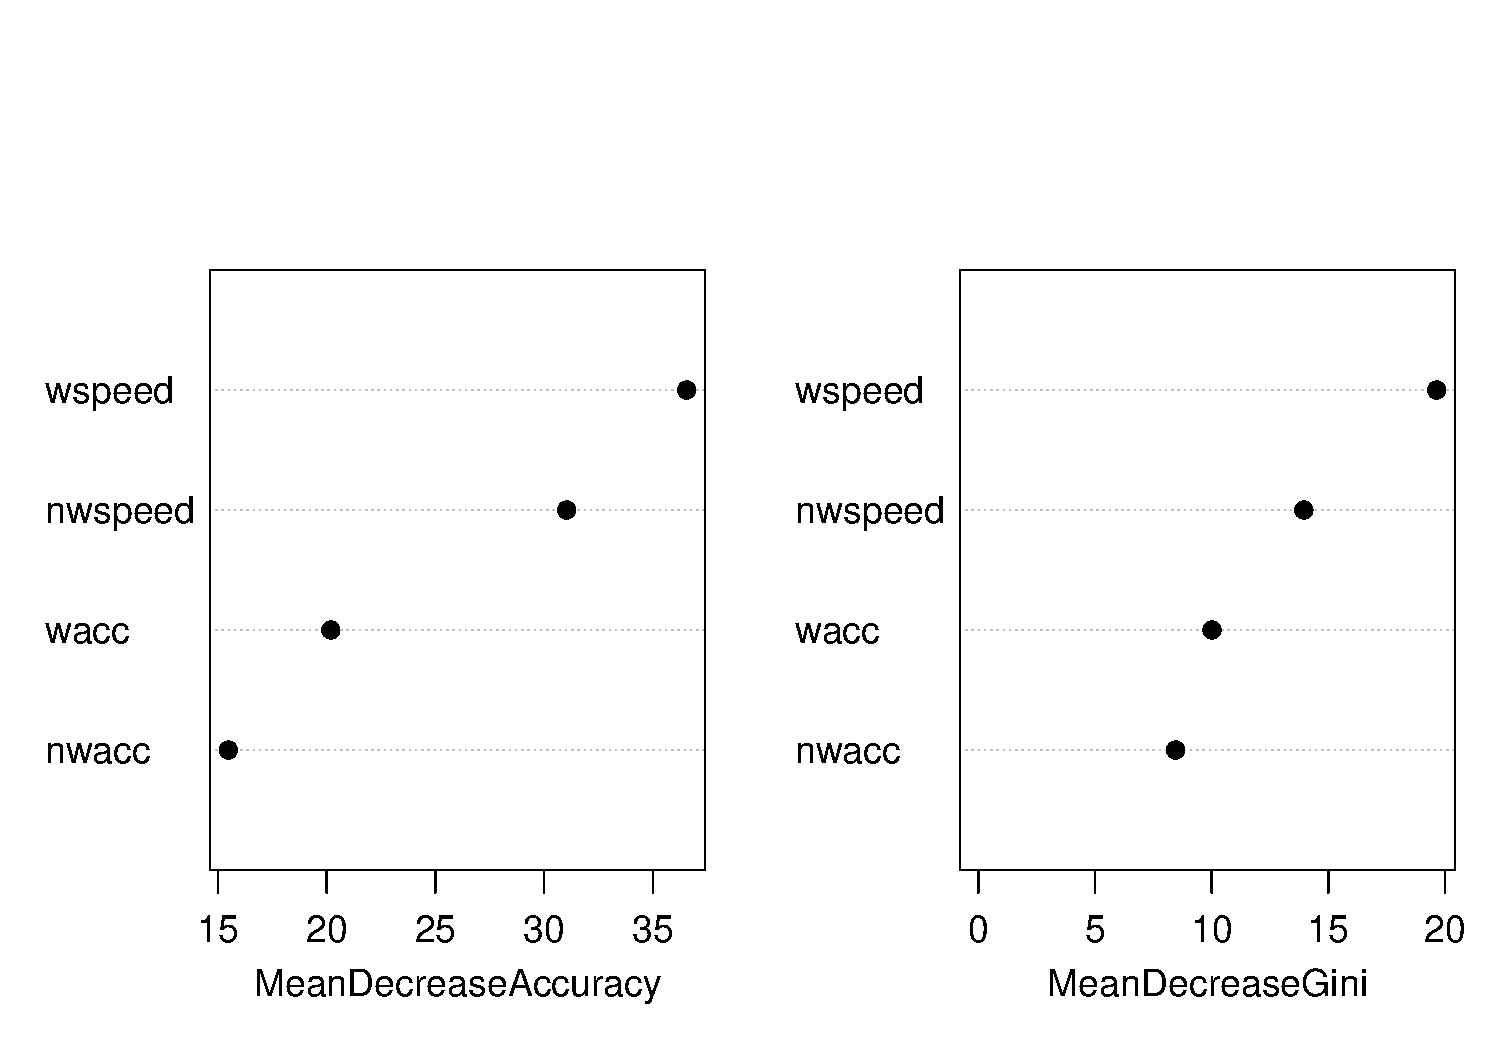
\includegraphics[width=1\textwidth]{/media/data/dyslexia_project/plot/f_class.pdf}
% \caption{Classification tree with DDE scores. Variable importance.}
% \label{fig:14}
% \end{figure} 

% Performing the classification with WISC subscales we obtain the following result:
% \begin{verbatim}
% Type of random forest: classification
%                      Number of trees: 500
% No. of variables tried at each split: 2
%         OOB estimate of  error rate: 58.14%
% Confusion matrix:
%    1 2  3 class.error
% 1 27 1 14   0.3571429
% 2  5 1  8   0.9285714
% 3 20 2  8   0.7333333
% \end{verbatim}

% Now we try the following approach in order to seek for a relationship
% between WISC subscales a DDE scores:
% \begin{enumerate}
% \item we fit a random forest model with classification trees on WISC
%   subscales considering only classes 1 (low dyslexia) and 3 (high
%   dyslexia).
% \item we select the most important variables.
% \item we fit a random forest model with regression trees with DDE
%   speed score (word/non-word) as response and selected WISC subscales
%   as regressors.
% \item we fit the model at Step 3. to the full database, in order to
%   check if the selected variables correctly predict the class 1
%   (medium dyslexia) scores.
% \end{enumerate}

% \paragraph{DDE Word Reading Speed Scores}
% \mbox{}\\
% First step:
% \begin{verbatim}
% Type of random forest: classification
%                      Number of trees: 500
% No. of variables tried at each split: 2

%         OOB estimate of  error rate: 48.61%
% Confusion matrix:
%    1  3 class.error
% 1 30 12   0.2857143
% 3 23  7   0.7666667
% \end{verbatim}
% \begin{figure}[h!] 
% \centering
% 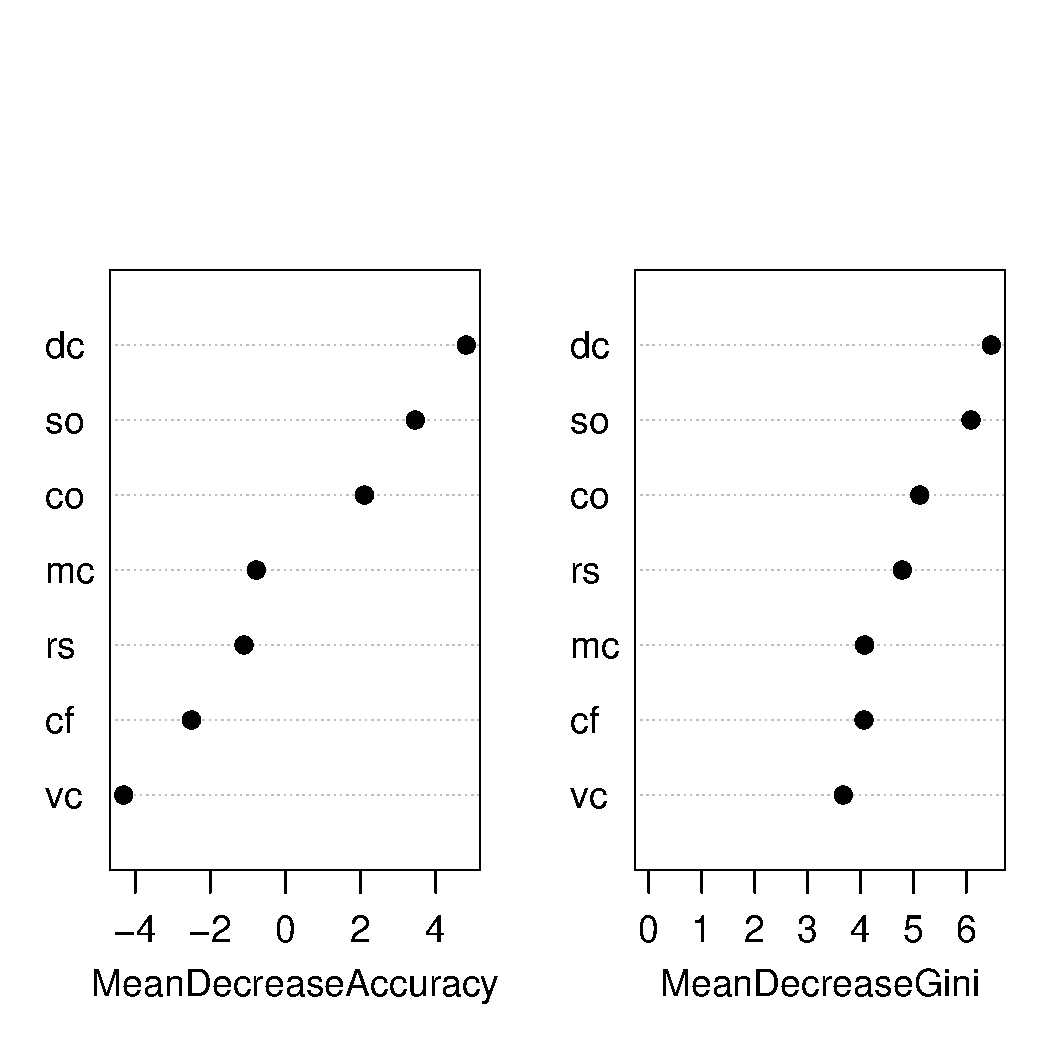
\includegraphics[width=1\textwidth]{/media/data/dyslexia_project/plot/fclass_wspeed.pdf}
% \caption{Classification tree of low (1) and high (3) dyslexia classes with WISC scores. Variable importance.}
% \label{fig:15}
% \end{figure}

% \clearpage

% Second step: Selected dc, so, co.\\
% Third step:
% \begin{verbatim}
% Type of random forest: regression
%                      Number of trees: 500  
% No. of variables tried at each split: 1

%           Mean of squared residuals: 8.060252
%                     % Var explained: -4.31
% \end{verbatim}
% Fourth step:
% \begin{figure}[h!] 
% \centering
% 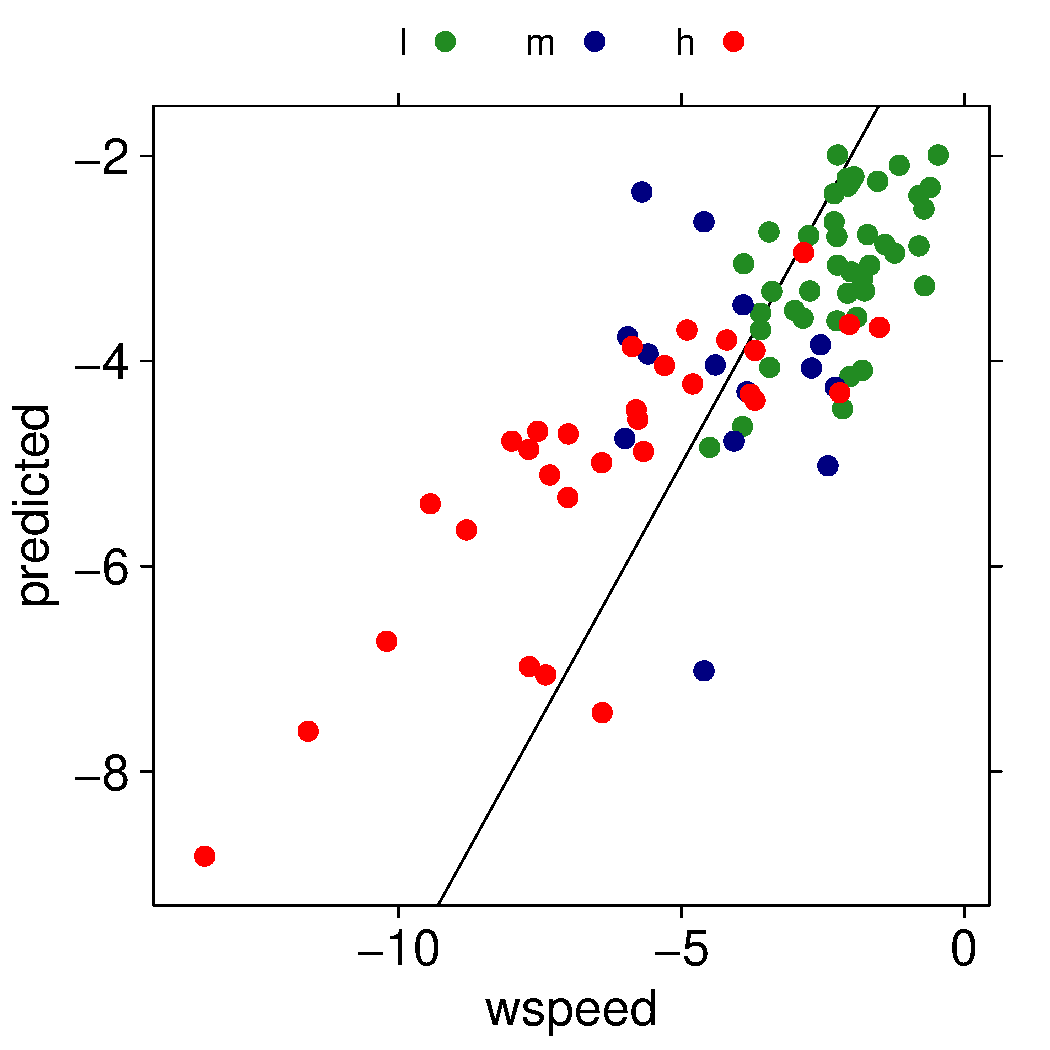
\includegraphics[width=1\textwidth]{/media/data/dyslexia_project/plot/predwspeed_plot.pdf}
% \caption{Predicted wspeed values with dc, so, co subscales as regressors.}
% \label{fig:16}
% \end{figure}

% \paragraph{DDE Non-Word Reading Speed Scores}
% \mbox{}\\
% Third step:
% \begin{verbatim}
% Type of random forest: regression
%                      Number of trees: 500
% No. of variables tried at each split: 1

%           Mean of squared residuals: 6.229219
%                     % Var explained: -15.4
% \end{verbatim}  
% Fourth step:
% \begin{figure}[h!] 
% \centering
% 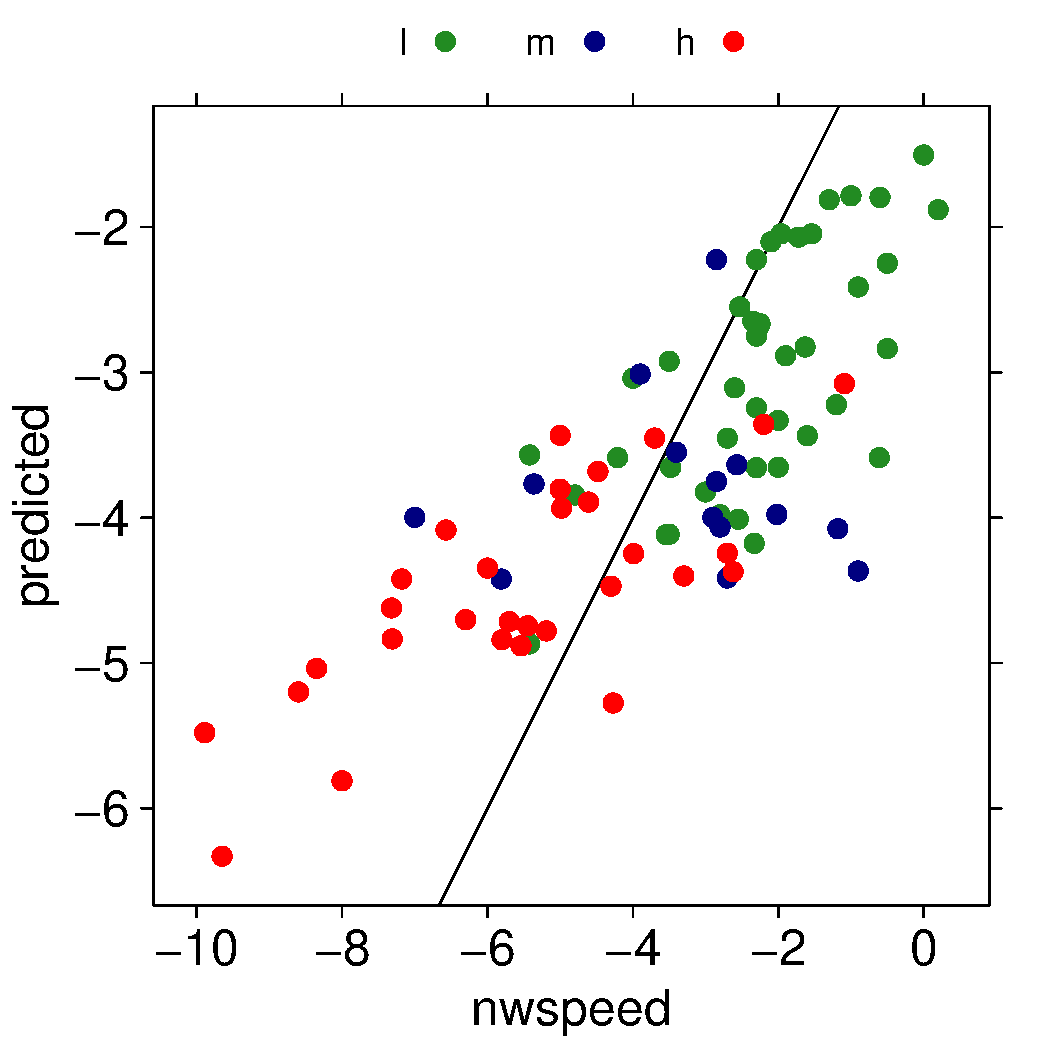
\includegraphics[width=1\textwidth]{/media/data/dyslexia_project/plot/prednwspeed_plot.pdf}
% \caption{Predicted nwspeed values with dc, so, co subscales as regressors.}
% \label{fig:17}
% \end{figure}

% \subsection{Logistic Regression}
% \begin{enumerate}
% \item We perform a generalized linear model with DSM5 classes as
%   response and $(wspeed+nwspeed)*(dc+so+mc+cf+vc+co+rs)$ as
%   regressors.
%   \begin{verbatim}
% Call:
% glm(formula = as.numeric(class) ~ (wspeed + nwspeed) * (dc + 
%     so + mc + cf + vc + co + rs), data = db)

% Deviance Residuals: 
%     Min       1Q   Median       3Q      Max  
% -1.0819  -0.3673   0.0273   0.2924   1.3917  

% Coefficients:
%               Estimate Std. Error t value Pr(>|t|)  
% (Intercept) -1.4527523  1.1786947  -1.233   0.2224  
% wspeed      -0.7192542  0.2955793  -2.433   0.0179 *
% nwspeed     -0.0379841  0.3332131  -0.114   0.9096  
% dc           0.0531177  0.0561646   0.946   0.3479  
% so           0.0509453  0.0702433   0.725   0.4710  
% mc          -0.0157737  0.0535120  -0.295   0.7692  
% cf           0.0120412  0.0661857   0.182   0.8562  
% vc           0.0458190  0.0642764   0.713   0.4786  
% co          -0.0205524  0.0689815  -0.298   0.7667  
% rs           0.0837888  0.0643954   1.301   0.1980  
% wspeed:dc    0.0278732  0.0156406   1.782   0.0796 .
% wspeed:so   -0.0003371  0.0160713  -0.021   0.9833  
% wspeed:mc   -0.0099392  0.0147529  -0.674   0.5030  
% wspeed:cf   -0.0080491  0.0165237  -0.487   0.6279  
% wspeed:vc    0.0340400  0.0220449   1.544   0.1276  
% wspeed:co   -0.0116266  0.0226920  -0.512   0.6102  
% wspeed:rs    0.0150460  0.0156261   0.963   0.3394  
% nwspeed:dc  -0.0042277  0.0170771  -0.248   0.8053  
% nwspeed:so   0.0010863  0.0235441   0.046   0.9633  
% nwspeed:mc   0.0090118  0.0167042   0.539   0.5915  
% nwspeed:cf   0.0119266  0.0175343   0.680   0.4989  
% nwspeed:vc  -0.0272551  0.0249071  -1.094   0.2781  
% nwspeed:co   0.0049547  0.0246277   0.201   0.8412  
% nwspeed:rs   0.0009999  0.0223444   0.045   0.9644  
% ---
% Signif. codes:  0 ‘***’ 0.001 ‘**’ 0.01 ‘*’ 0.05 ‘.’ 0.1 ‘ ’ 1

% (Dispersion parameter for gaussian family taken to be 0.346641)

%     Null deviance: 70.326  on 85  degrees of freedom
% Residual deviance: 21.492  on 62  degrees of freedom
% AIC: 174.8

% Number of Fisher Scoring iterations: 2
% \end{verbatim}
% \item We perform a generalized linear model as before, but only with
%   wspeed as DDE score.
% \begin{verbatim}
% Call:
% glm(formula = as.numeric(class) ~ (wspeed) * (dc + so + mc + 
%     cf + vc + co + rs), data = db)

% Deviance Residuals: 
%      Min        1Q    Median        3Q       Max  
% -1.09783  -0.38314  -0.01877   0.31199   1.46870  

% Coefficients:
%              Estimate Std. Error t value Pr(>|t|)   
% (Intercept) -1.536257   1.050852  -1.462  0.14824   
% wspeed      -0.763376   0.249875  -3.055  0.00318 **
% dc           0.062294   0.052323   1.191  0.23784   
% so           0.070691   0.061652   1.147  0.25545   
% mc          -0.025985   0.047962  -0.542  0.58970   
% cf           0.023843   0.059087   0.404  0.68779   
% vc           0.041189   0.063746   0.646  0.52030   
% co          -0.005472   0.061786  -0.089  0.92968   
% rs           0.061151   0.053304   1.147  0.25520   
% wspeed:dc    0.026036   0.011205   2.324  0.02306 * 
% wspeed:so   -0.002213   0.011844  -0.187  0.85229   
% wspeed:mc   -0.006564   0.012072  -0.544  0.58836   
% wspeed:cf    0.005038   0.013625   0.370  0.71265   
% wspeed:vc    0.005968   0.014774   0.404  0.68749   
% wspeed:co    0.004074   0.016744   0.243  0.80846   
% wspeed:rs    0.013701   0.010941   1.252  0.21464   
% ---
% Signif. codes:  0 ‘***’ 0.001 ‘**’ 0.01 ‘*’ 0.05 ‘.’ 0.1 ‘ ’ 1

% (Dispersion parameter for gaussian family taken to be 0.3738487)

%     Null deviance: 70.326  on 85  degrees of freedom
% Residual deviance: 26.169  on 70  degrees of freedom
% AIC: 175.74

% Number of Fisher Scoring iterations: 2
% \end{verbatim}
% \item We perform a generalized linear model as before, but only with
%   nwspeed as DDE score.
% \begin{verbatim}
% Call:
% glm(formula = as.numeric(class) ~ (nwspeed) * (dc + so + mc + 
%     cf + vc + co + rs), data = db)

% Deviance Residuals: 
%      Min        1Q    Median        3Q       Max  
% -1.45153  -0.48069  -0.03166   0.46398   1.52062  

% Coefficients:
%               Estimate Std. Error t value Pr(>|t|)  
% (Intercept) -0.8018996  1.2816080  -0.626   0.5335  
% nwspeed     -0.6344651  0.3267787  -1.942   0.0562 .
% dc          -0.0167730  0.0632053  -0.265   0.7915  
% so           0.1513009  0.0823838   1.837   0.0705 .
% mc          -0.0105356  0.0597755  -0.176   0.8606  
% cf           0.0671982  0.0723314   0.929   0.3561  
% vc           0.0066307  0.0703881   0.094   0.9252  
% co          -0.0253525  0.0765273  -0.331   0.7414  
% rs           0.0126075  0.0752521   0.168   0.8674  
% nwspeed:dc  -0.0008382  0.0146107  -0.057   0.9544  
% nwspeed:so   0.0260926  0.0205275   1.271   0.2079  
% nwspeed:mc  -0.0004094  0.0161121  -0.025   0.9798  
% nwspeed:cf   0.0178704  0.0167581   1.066   0.2899  
% nwspeed:vc   0.0084209  0.0194769   0.432   0.6668  
% nwspeed:co  -0.0113936  0.0211721  -0.538   0.5922  
% nwspeed:rs   0.0010554  0.0183193   0.058   0.9542  
% ---
% Signif. codes:  0 ‘***’ 0.001 ‘**’ 0.01 ‘*’ 0.05 ‘.’ 0.1 ‘ ’ 1

% (Dispersion parameter for gaussian family taken to be 0.5281967)

%     Null deviance: 70.326  on 85  degrees of freedom
% Residual deviance: 36.974  on 70  degrees of freedom
% AIC: 205.46

% Number of Fisher Scoring iterations: 2
% \end{verbatim}
% \end{enumerate}
% It is worth observing the significance of the interaction $wspeed*dc$
% ($p<0.05$) in the second model. $dc$ is the most important variable
% selected by the random forest model implemented in the previous
% subsection. Moreover we can observe the lower significance ($p<0.1$)
% of the subscale $so$ in the third model. $so$ is the second subscale
% value selected by the random forest model implemented in the previous
% subsection.


% \section{Multinomial Logistic Regression}
% \begin{enumerate}
% \item Regressors: dde variables (wspeed,nwspeed,wacc,nwacc). Reference
%   level $\longrightarrow$ class $3$.
% \begin{verbatim}
% Call:
% multinom(formula = form.dde, data = db.tmp)

% Coefficients:
%   (Intercept)    wspeed   nwspeed      wacc    nwacc
% 1   197.58085 17.493015 20.179414 18.755749 16.97987
% 2    72.10549  4.504629  6.428822  6.531223  6.56515

% Std. Errors:
%   (Intercept)   wspeed   nwspeed      wacc    nwacc
% 1   104.88858 9.866885 11.586665 10.739339 9.701778
% 2    57.39051 4.164916  5.752461  6.223839 6.106167

% Residual Deviance: 0.8815825 
% AIC: 20.88158 

% P-values:
%   (Intercept)     wspeed    nwspeed      wacc      nwacc
% 1  0.05960269 0.07624501 0.08157729 0.0807323 0.08008696
% 2  0.20897067 0.27944577 0.26374742 0.2939995 0.28229995
% \end{verbatim}
% \begin{figure}[h!] 
% \centering
% 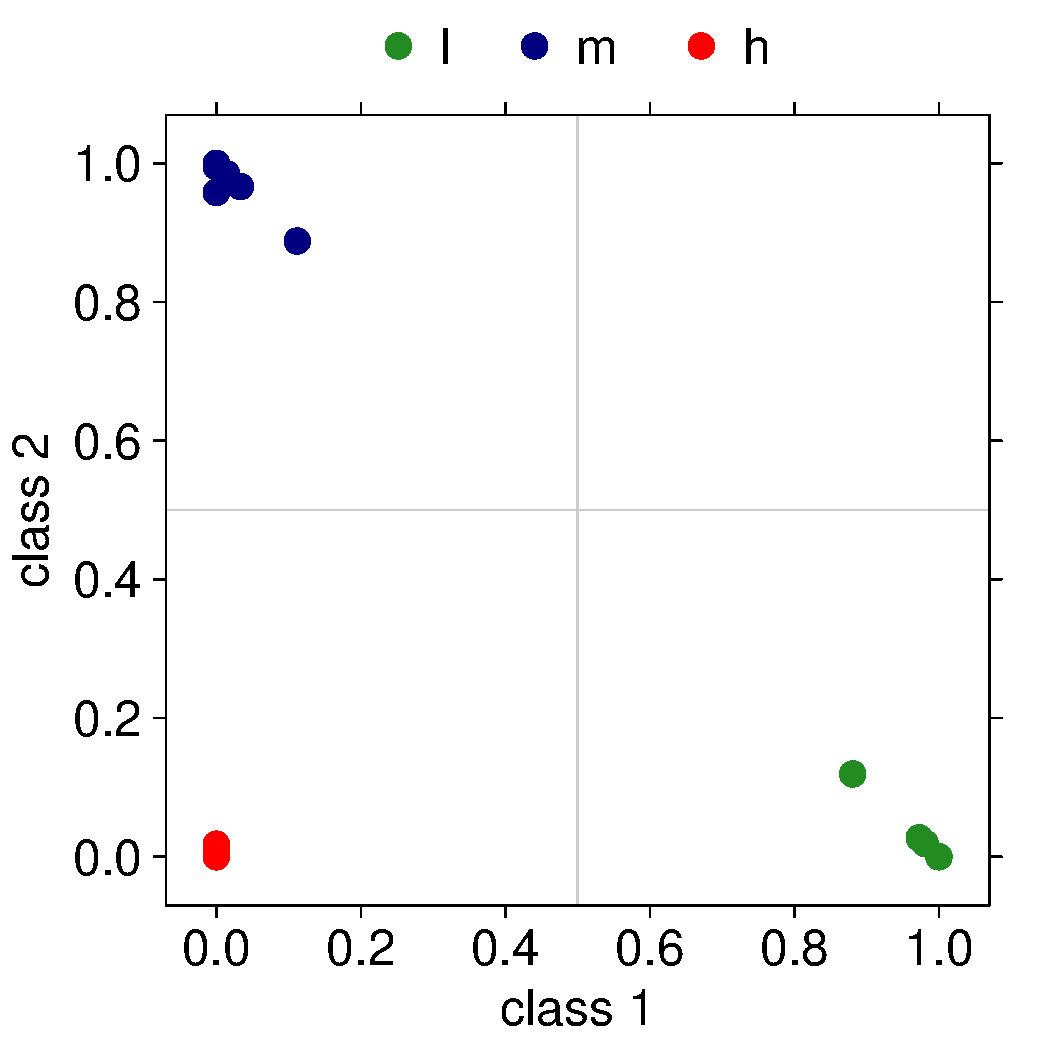
\includegraphics[width=1\textwidth]{/media/data/dyslexia_project/plot/multGLM_dde.pdf}
% \caption{Multinomial logistic regression on dyslexia class, with dde scores as regressors.}
% \label{fig:18}
% \end{figure}  

% \clearpage

% \item Regressors: dde variables:wisc subscales
%   (dc+cf+rs+so+vc+co+mc). Reference level $\longrightarrow$ class $3$.
% \begin{verbatim}
% Call:
% multinom(formula = form.inter, data = db.tmp)

% Coefficients:
%   (Intercept)  wspeed:dc  wspeed:cf  wspeed:rs wspeed:mc wspeed:so wspeed:vc
% 1   155.71909  0.3342648 0.03952001  0.9264321 2.2657407 0.8902855 -1.509521
% 2    70.17509 -0.8217690 2.15442465 -3.8670681 0.3964486 6.0207881 -2.854898
%    wspeed:co    wacc:dc   wacc:cf   wacc:rs  wacc:mc   wacc:so   wacc:vc
% 1 -0.0667730 -2.1048418 -2.814648 0.8747144 1.610395  2.413544 -2.480102
% 2 -0.5481724 -0.5554065 -5.768567 3.5798315 3.703040 -5.383504  2.095209
%    wacc:co nwspeed:dc nwspeed:cf nwspeed:rs nwspeed:mc nwspeed:so nwspeed:vc
% 1 1.881738 -0.7359609  1.5059307 -0.9581549  -1.447987 -0.6769544   2.874844
% 2 2.727121 -0.2459587 -0.6291299  3.3131139  -1.736066 -5.4680130   4.315976
%   nwspeed:co nwacc:dc  nwacc:cf   nwacc:rs   nwacc:mc  nwacc:so   nwacc:vc
% 1  0.1885891 2.632224 0.5703178 -0.7755046 -0.9244619 -1.285881  3.8711319
% 2  1.3454552 3.770200 4.9178314 -4.2213342 -1.5216561  3.250182 -0.5353119
%    nwacc:co
% 1 -2.097886
% 2 -4.677192

% Std. Errors:
%   (Intercept) wspeed:dc wspeed:cf wspeed:rs wspeed:mc wspeed:so wspeed:vc
% 1    198.3953  619.0846 1573.2037  520.3707 1155.7102  596.9785 1320.9672
% 2    181.1330  377.2129  318.4729  345.0649  441.5142  427.4253  481.9091
%   wspeed:co  wacc:dc  wacc:cf  wacc:rs  wacc:mc   wacc:so   wacc:vc   wacc:co
% 1  402.7968 414.7655 697.8195 518.0233 373.2299 1708.0067  461.8061 1212.9684
% 2  639.4655 684.3562 201.6864 539.2540 822.2969  952.6766 1356.6554  738.0164
%   nwspeed:dc nwspeed:cf nwspeed:rs nwspeed:mc nwspeed:so nwspeed:vc nwspeed:co
% 1   363.9444   675.9214   781.5355   648.1829   370.0346   505.6632   457.1549
% 2   421.8806   870.6919   256.1981   345.1745   253.9231   619.9579   448.3060
%   nwacc:dc nwacc:cf nwacc:rs nwacc:mc nwacc:so nwacc:vc  nwacc:co
% 1 993.3434  209.252 751.7241 784.8282 435.3508 305.2842  490.4145
% 2 902.9500 1322.052 653.5004 581.7775 908.1572 564.2960 1412.9238

% Residual Deviance: 0.0001232419 
% AIC: 116.0001 


% P-values:
%   (Intercept) wspeed:dc wspeed:cf wspeed:rs wspeed:mc wspeed:so wspeed:vc
% 1   0.4325164 0.9995692 0.9999800 0.9985795 0.9984358 0.9988101 0.9990882
% 2   0.6984430 0.9982618 0.9946025 0.9910585 0.9992836 0.9887612 0.9952732
%   wspeed:co   wacc:dc   wacc:cf   wacc:rs   wacc:mc   wacc:so   wacc:vc
% 1 0.9998677 0.9959509 0.9967817 0.9986527 0.9965573 0.9988725 0.9957150
% 2 0.9993160 0.9993525 0.9771823 0.9947033 0.9964069 0.9954912 0.9987678
%     wacc:co nwspeed:dc nwspeed:cf nwspeed:rs nwspeed:mc nwspeed:so nwspeed:vc
% 1 0.9987622  0.9983865  0.9982223  0.9990218  0.9982176  0.9985403  0.9954638
% 2 0.9970517  0.9995348  0.9994235  0.9896822  0.9959870  0.9828196  0.9944454
%   nwspeed:co  nwacc:dc  nwacc:cf  nwacc:rs  nwacc:mc  nwacc:so  nwacc:vc
% 1  0.9996709 0.9978857 0.9978254 0.9991769 0.9990602 0.9976433 0.9898828
% 2  0.9976054 0.9966685 0.9970320 0.9948460 0.9979131 0.9971445 0.9992431
%    nwacc:co
% 1 0.9965868
% 2 0.9973588
% \end{verbatim}

% \begin{figure}[h!] 
% \centering
% 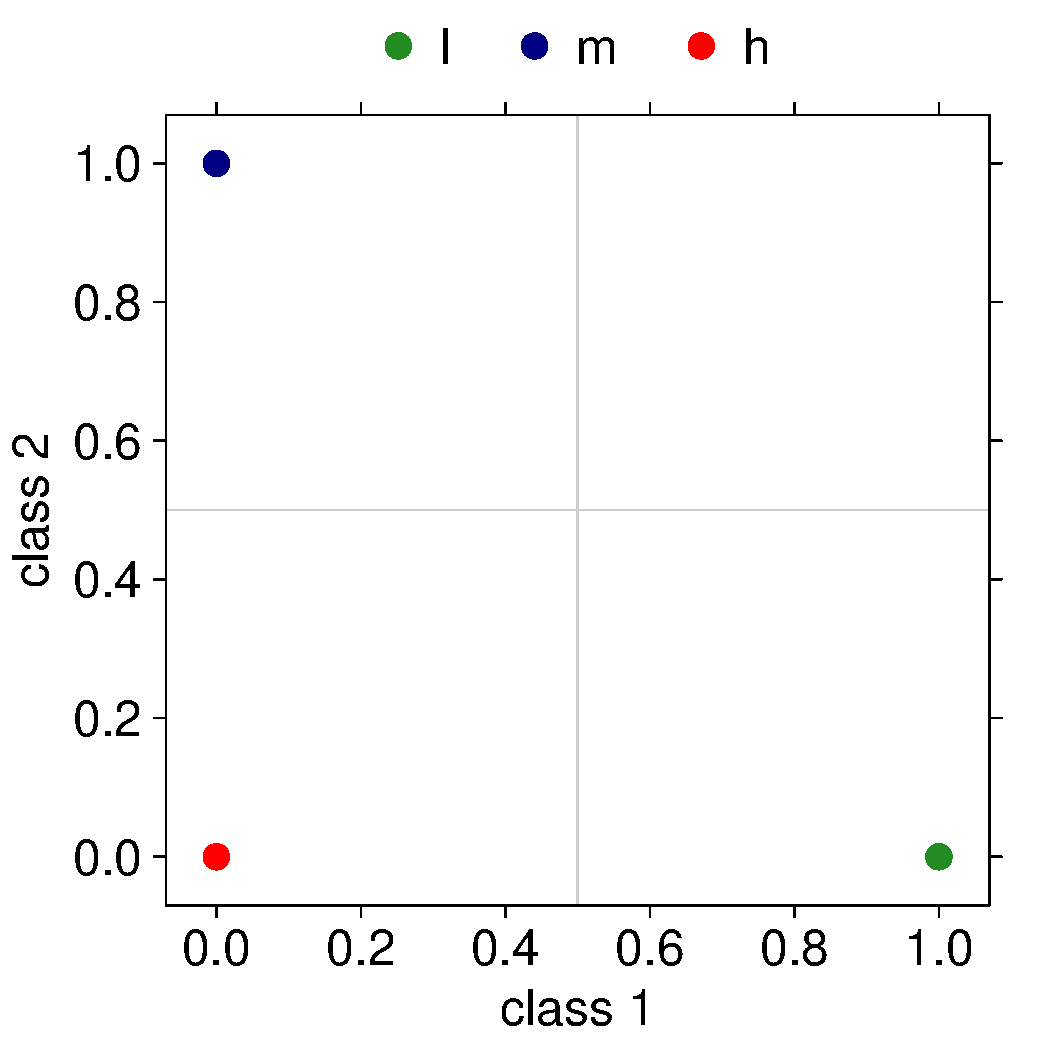
\includegraphics[width=1\textwidth]{/media/data/dyslexia_project/plot/multGLM_inter.pdf}
% \caption{Multinomial logistic regression on dyslexia class, with
%   interaction dde scores and wisc subscales as regressors.}
% \label{fig:19}
% \end{figure}  

% \clearpage

% \item Regressors: dde speed scores $*$ visual wisc subscales (dc+cf+rs).
% \begin{verbatim}
% Call:
% multinom(formula = form.visivispeed, data = db.tmp)

% Coefficients:
%   (Intercept)  wspeed:dc wspeed:cf  wspeed:rs  nwspeed:dc nwspeed:cf nwspeed:rs
% 1    6.277681 0.00611342 0.2584666 -0.1146242  0.06079504 -0.1850473  0.1639073
% 2    2.039740 0.02950453 0.1529593 -0.1650891 -0.01074398 -0.1737438  0.2351008

% Std. Errors:
%   (Intercept)  wspeed:dc  wspeed:cf  wspeed:rs nwspeed:dc nwspeed:cf nwspeed:rs
% 1    1.298233 0.08365329 0.09530742 0.12434004 0.07698627 0.07868204  0.1160773
% 2    1.112825 0.05578426 0.06819754 0.08080758 0.06453172 0.07505726  0.1043742

% Residual Deviance: 103.2073 
% AIC: 131.2073 

% P-values:
%    (Intercept) wspeed:dc   wspeed:cf  wspeed:rs nwspeed:dc nwspeed:cf
% 1 1.327723e-06 0.9417421 0.006689371 0.35660142  0.4297108 0.01868099
% 2 6.681165e-02 0.5968719 0.024904171 0.04105346  0.8677702 0.02062300
%   nwspeed:rs
% 1  0.1579344
% 2  0.0242920
% \end{verbatim}
% \begin{figure}[h!] 
% \centering
% 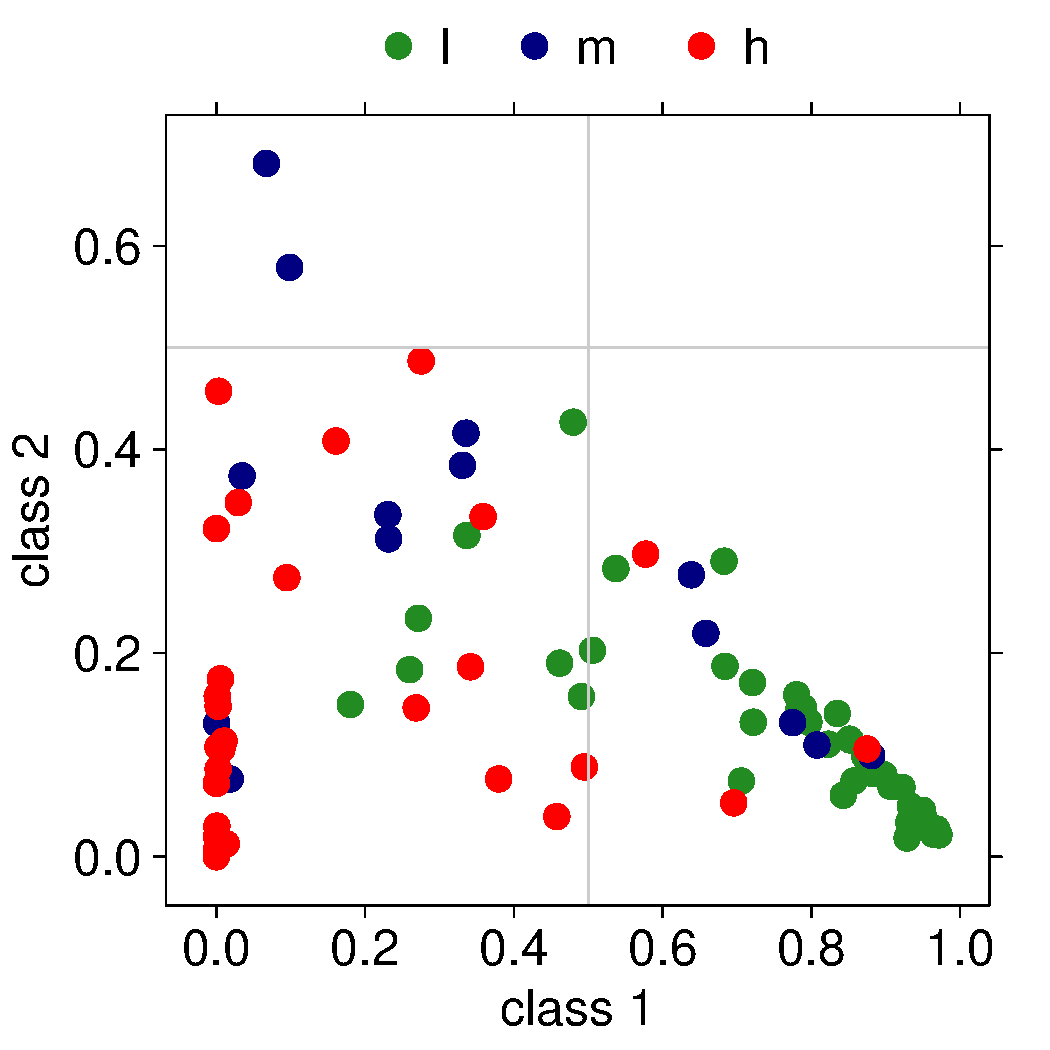
\includegraphics[width=1\textwidth]{/media/data/dyslexia_project/plot/multGLM_visivi.pdf}
% \caption{Multinomial logistic regression on dyslexia class, with
%   interaction dde speed scores and visual wisc subscales as regressors.}
% \label{fig:21}
% \end{figure}

% \clearpage

% \item Regressors: dde speed scores $*$ verbal wisc subscales (so+vc+co).
% \begin{verbatim}
% Call:
% multinom(formula = form.verbspeed, data = db.tmp)

% Coefficients:
%   (Intercept)    wspeed:so  wspeed:vc wspeed:co  nwspeed:so nwspeed:vc
% 1    6.649187 0.1411143522 -0.1372634 0.1040200 -0.06918093  0.2415311
% 2    2.224401 0.0008399367 -0.2385547 0.2326216  0.02172425  0.3298946
%   nwspeed:co
% 1 -0.1119064
% 2 -0.2798262

% Std. Errors:
%   (Intercept)  wspeed:so wspeed:vc wspeed:co nwspeed:so nwspeed:vc nwspeed:co
% 1    1.361804 0.12371457 0.1244158 0.1449235  0.1379826  0.1392925  0.1556190
% 2    1.248451 0.07401035 0.1072877 0.1242906  0.1083624  0.1344208  0.1515837

% Residual Deviance: 97.91408 
% AIC: 125.9141 

% P-values:
%    (Intercept) wspeed:so  wspeed:vc  wspeed:co nwspeed:so nwspeed:vc nwspeed:co
% 1 1.046801e-06 0.2540179 0.26991283 0.47290648  0.6161076 0.08292065 0.47207613
% 2 7.479351e-02 0.9909451 0.02618173 0.06126276  0.8411069 0.01412014 0.06488965
% \end{verbatim}
% \begin{figure}[h!] 
% \centering
% 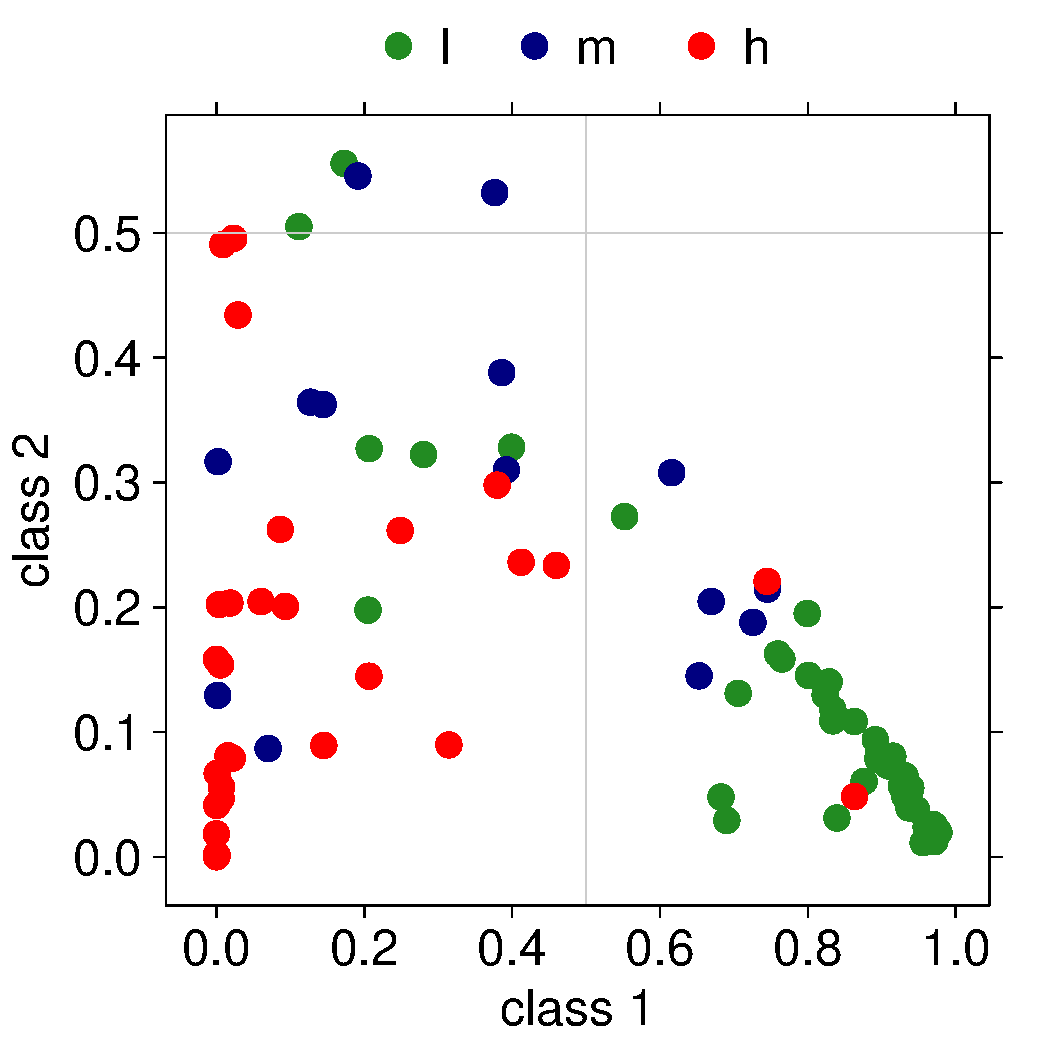
\includegraphics[width=1\textwidth]{/media/data/dyslexia_project/plot/multGLM_verbali.pdf}
% \caption{Multinomial logistic regression on dyslexia class, with
%   interaction dde speed scores and verbal wisc subscales as regressors.}
% \label{fig:22}
% \end{figure}

% \clearpage

% \item Regressors: wisc subscales
%   (dc+cf+rs+so+vc+co+mc). Reference level $\longrightarrow$ class $3$.
% \begin{verbatim}
% Call:
% multinom(formula = form.sub, data = db.tmp)

% Coefficients:
%   (Intercept)          dc          cf         rs           mc          so
% 1    1.341380 -0.07089792 -0.05945828 0.12023871  0.009459909 -0.18255369
% 2   -3.057193 -0.04641101  0.10046204 0.04019967 -0.036906151 -0.02193856
%             vc        co
% 1 -0.077716873 0.1542340
% 2  0.008973166 0.1838802

% Std. Errors:
%   (Intercept)         dc        cf        rs         mc        so        vc
% 1    1.823957 0.09420951 0.1087047 0.1044373 0.09065468 0.1228189 0.1220454
% 2    2.445674 0.12552842 0.1405156 0.1455718 0.12152918 0.1679099 0.1723151
%          co
% 1 0.1238968
% 2 0.1650733

% Residual Deviance: 164.6416 
% AIC: 196.6416 

% P-values:
%   (Intercept)        dc        cf        rs        mc        so        vc
% 1   0.4620820 0.4517169 0.5843989 0.2496088 0.9168908 0.1371825 0.5242638
% 2   0.2112846 0.7115873 0.4746380 0.7824327 0.7613706 0.8960469 0.9584696
%          co
% 1 0.2131839
% 2 0.2653091
% \end{verbatim}

% \begin{figure}[h!] 
% \centering
% 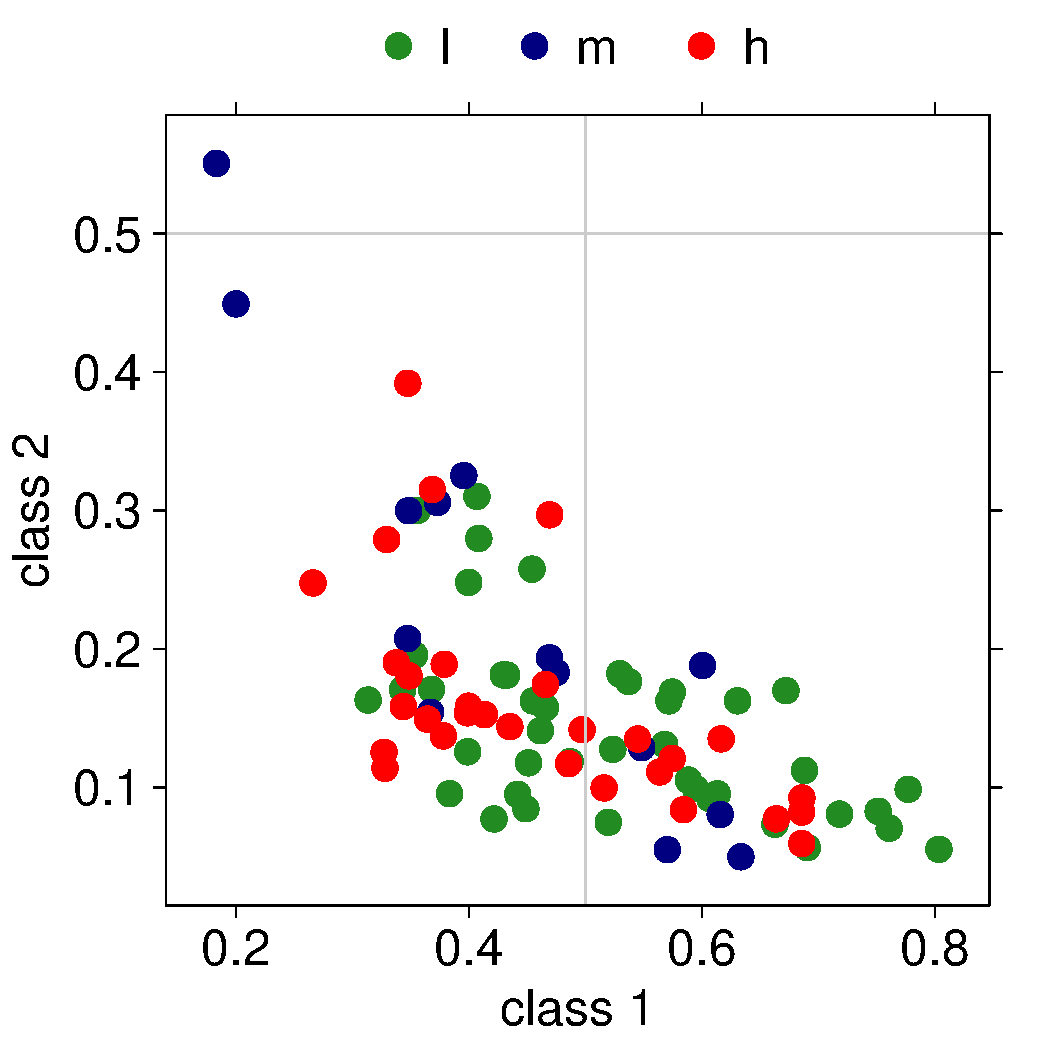
\includegraphics[width=1\textwidth]{/media/data/dyslexia_project/plot/multGLM_sub.pdf}
% \caption{Multinomial logistic regression on dyslexia class, with
%   wisc subscales as regressors.}
% \label{fig:20}
% \end{figure}
% \end{enumerate}

% \clearpage

% If we reduce to only consider classes $1$ and $3$ we obtain:
% \begin{itemize}
% \item $class~(wacc+nwacc+wspeed+nwspeed)*(dc+so+mc+cf+vc+co+rs)$
% \begin{verbatim}
% Warning messages:
% 1: glm.fit: algorithm did not converge 
% 2: glm.fit: fitted probabilities numerically 0 or 1 occurred
% \end{verbatim}
% \item $class~wspeed+nwspeed+wacc+nwacc$
% \begin{verbatim}
% Call:
% glm(formula = form, family = binomial, data = data)

% Deviance Residuals: 
%        Min          1Q      Median          3Q         Max  
% -3.414e-05  -2.100e-08   2.100e-08   2.100e-08   4.329e-05  

% Coefficients:
%              Estimate Std. Error z value Pr(>|z|)
% (Intercept)    170.93  106509.49   0.002    0.999
% wspeed          12.42   22953.48   0.001    1.000
% nwspeed         15.27   19789.85   0.001    0.999
% wacc            16.20   11885.89   0.001    0.999
% nwacc           16.76   14639.62   0.001    0.999

% (Dispersion parameter for binomial family taken to be 1)

%     Null deviance: 9.7804e+01  on 71  degrees of freedom
% Residual deviance: 4.5129e-09  on 67  degrees of freedom
% AIC: 10

% Number of Fisher Scoring iterations: 25
% \end{verbatim}
% \item $class~(wspeed+wacc+nwspeed+nwacc):(dc+cf+rs+mc+so+vc+co)$
% \begin{verbatim}
% Warning messages:
% 1: glm.fit: algorithm did not converge 
% 2: glm.fit: fitted probabilities numerically 0 or 1 occurred 
% \end{verbatim}
% \item $class~dc+cf+rs+mc+so+vc+co$
% \begin{verbatim}
% Call:
% glm(formula = form, family = binomial, data = data)

% Deviance Residuals: 
%     Min       1Q   Median       3Q      Max  
% -1.6764  -1.1531   0.7178   1.0841   1.3691  

% Coefficients:
%              Estimate Std. Error z value Pr(>|z|)
% (Intercept)  1.643483   2.026490   0.811    0.417
% dc          -0.064009   0.094734  -0.676    0.499
% cf          -0.079863   0.114484  -0.698    0.485
% rs           0.121840   0.101854   1.196    0.232
% mc           0.008063   0.089418   0.090    0.928
% so          -0.181098   0.127121  -1.425    0.154
% vc          -0.076115   0.129030  -0.590    0.555
% co           0.130424   0.121668   1.072    0.284

% (Dispersion parameter for binomial family taken to be 1)

%     Null deviance: 97.804  on 71  degrees of freedom
% Residual deviance: 92.919  on 64  degrees of freedom
% AIC: 108.92

% Number of Fisher Scoring iterations: 4
% \end{verbatim}

% \item $class~(wspeed+nwspeed):(dc+cf+rs)$ (VISIVI)
% \begin{verbatim}
% Call:
% glm(formula = form, family = binomial, data = data)

% Deviance Residuals: 
%     Min       1Q   Median       3Q      Max  
% -2.9962  -0.1195   0.1354   0.3802   1.6085  

% Coefficients:
%             Estimate Std. Error z value Pr(>|z|)    
% (Intercept)  6.42550    1.67242   3.842 0.000122 ***
% wspeed:dc   -0.04907    0.08932  -0.549 0.582720    
% wspeed:cf    0.29366    0.11144   2.635 0.008408 ** 
% wspeed:rs   -0.11524    0.12159  -0.948 0.343227    
% nwspeed:dc   0.11803    0.08430   1.400 0.161474    
% nwspeed:cf  -0.19764    0.08638  -2.288 0.022134 *  
% nwspeed:rs   0.14482    0.11464   1.263 0.206504    
% ---
% Signif. codes:  0 ‘***’ 0.001 ‘**’ 0.01 ‘*’ 0.05 ‘.’ 0.1 ‘ ’ 1

% (Dispersion parameter for binomial family taken to be 1)

%     Null deviance: 97.804  on 71  degrees of freedom
% Residual deviance: 38.843  on 65  degrees of freedom
% AIC: 52.843

% Number of Fisher Scoring iterations: 7
% \end{verbatim}

% \item $class~(wspeed+nwspeed):(so+vc+co)$ (VERBALI)
% \begin{verbatim}
% Call:
% glm(formula = form, family = binomial, data = data)

% Deviance Residuals: 
%     Min       1Q   Median       3Q      Max  
% -2.6944  -0.2183   0.1092   0.3165   1.7802  

% Coefficients:
%             Estimate Std. Error z value Pr(>|z|)    
% (Intercept)  6.43340    1.59738   4.027 5.64e-05 ***
% wspeed:so    0.11347    0.12399   0.915   0.3601    
% wspeed:vc   -0.17754    0.14304  -1.241   0.2145    
% wspeed:co    0.14524    0.16208   0.896   0.3702    
% nwspeed:so  -0.07763    0.13232  -0.587   0.5574    
% nwspeed:vc   0.29298    0.16694   1.755   0.0793 .  
% nwspeed:co  -0.13971    0.17006  -0.821   0.4114    
% ---
% Signif. codes:  0 ‘***’ 0.001 ‘**’ 0.01 ‘*’ 0.05 ‘.’ 0.1 ‘ ’ 1

% (Dispersion parameter for binomial family taken to be 1)

%     Null deviance: 97.804  on 71  degrees of freedom
% Residual deviance: 35.733  on 65  degrees of freedom
% AIC: 49.733

% Number of Fisher Scoring iterations: 7
% \end{verbatim}
% \end{itemize}


\section{Method}

\subsection{Participants}
The present study involved $86$ subjects with age ranging from $86$
months ($\sim 7$ years) to $205$ months ($\sim 17$ years). At the time
of the recruitment the mean age of the subjects was $144.08$ months
($\sim 12$ years), with a standard deviation of $30.90$ ($\sim 2.60$).
Reclutamento: essere sotto le 2 deviazioni standard in almeno un
valore della dde e/o rientrare nella diagnosi della dislessia con la
lettura di brano.\\
\emph{Osservazione:} quali sono i criteri di inclusione? Se il
criterio di inclusione e' essere carente in uno degli score della dde
(quindi punteggio <=-2.0), allora i soggetti 509 e 734 perch\'e sono
stati reclutati?
\begin{verbatim}
    id class comorb age wspeed wacc nwspeed nwacc errtc errsub QI VCI PRI WMI
58 509     0      0 190  -1.15    1   -1.72   1.0     5      0 96 102  92 115
77 734     0      0 146  -0.60    1   -0.90   0.6     0      0 95 100  99 115
   PSI dc so mc cf vc co rs errtot perc.errtc perc.errsub bakker
58  97  8  9 12 10  8 13  9      5          1           0      P
77  85 10 11 15  5 10 12 10      0          0           0      M
\end{verbatim}


\subsection{Procedure}
Since we based our classification on several criteria, such as DSM-V,
clinical evaluation and DDE, firstly we proceeded with a qualitative
data visualization, trying to assess the relationship between the
classes and the DDE scores. We plotted the accuracy (both for words
and non-words) against the speed (both for words and non-words) and we
observed the general trend divided by class. The general trend for all
the three classes is decreasing when plotting non-word accuracy
against non-word speed. Subject ``673'' was clearly outside the
distribution and we decided to discard it, treating it as an
outlier. Hence we reduced our database from 96 subjects to 95
subjects. Moreover it can be observed that the subjects of third
class, that of the subjects classified as ``severe'', assume spreader
values than the subjects classified as ``low'' and ``medium''. It is
straightforward that the classes with a lower impairment tend to
display subjects closer to each other and with a less steep decreasing
trend. When inspecting the classes distribution in the case of the
plot of word accuracy against word speed we observed that the trend of
the ``severe'' class is increasing, whereas the trend of both the
``low'' and ``medium'' classes is increasing. Hence, higher the
accuracy, higher the speed for the third class, while higher the
accuracy, lower the speed for the first and second classes. It is
straightforward that the values of the third class tend to be lower
than the other and in most cases lower than the cutoff of $-2.0$. In
this case too it was possible to observe that the two higher classes
tend to be closer to each other, while the third class spreads its
values assuming a wider range of values.\\
From these graphs we could observe that accuracy and speed modulate
the three classes and show that classes 0 and 1 behave in the same way
and assume close values. It can be hypothesized that class 1 can be
seen as a class 0, dividing the dataset into a two-classes
classification. In order to state that the Kruskal-Wallis test was
made. The Kruskal-Wallis test is a non-parametric method for testing
whether samples originate from the same distribution. We tested the
DDE scores for classes 0 and 1 and for classes 1 and 2
respectively. We expected to have the same distribution (accept the
null hypothesis) in the case of classes 0 and 1 and to reject the null
hypothesis, hence statistically different distributions between
classes 1 and 2. The results obtained are shown in
Tables~\ref{tab:1},\ref{tab:2}. As we can observe the results are in
line with what we expected. In fact we can reject the alternative
hypothesis given the p-values in Table~\ref{tab:1}, hence the DDE
scores correspondent to classes 0 and 1 have the same
distribution. Moreover, from the p-values in Table~\ref{tab:2}, we
accept the alternative hypothesis stating that the DDE scores
correspondent to classes 1 and 2 have different distribution.

\begin{table}[ht]
\centering
\begin{tabular}{lrr}
  \hline
dde.score & chi.sq & p.value \\ 
  \hline
word speed & 3.91 & 0.05 \\ 
  non-word speed & 3.12 & 0.08 \\ 
  word accuracy & 3.89 & 0.05 \\ 
  non-word accuracy & 0.59 & 0.44 \\ 
   \hline
\end{tabular}
\caption{Classes 0 and 1.}
\label{tab:1}
\end{table}

\begin{table}[ht]
\centering
\begin{tabular}{lrr}
  \hline
dde.score & chi.sq & p.value \\ 
  \hline
word speed & 7.880 & 0.005 \\ 
  non-word speed & 9.920 & 0.002 \\ 
  word accuracy & 5.920 & 0.015 \\ 
  non-word accuracy & 4.860 & 0.028 \\ 
   \hline
\end{tabular}
\caption{Classes 1 and 2.}
\label{tab:2}
\end{table}

We merged the ``low'' and ``medium'' classes and we test the new
classification, in order to prove that the distribution still differ
with the new classification, hence we run the Kruskal-Wallis test
again. Results are shown in Table~\ref{tab:3}.

\begin{table}[ht]
\centering
\begin{tabular}{lrr}
  \hline
dde.score & chi.sq & p.value \\ 
  \hline
word speed & 37.73 & <0.001 \\ 
  non-word speed & 31.70 & <0.001 \\ 
  word accuracy & 22.63 & <0.001 \\ 
  non-word accuracy & 15.70 & <0.001 \\ 
   \hline
\end{tabular}
\caption{Merged 0 and 1 classes and class 2.}
\label{tab:3}
\end{table}
This merge could be done, and we obtained a dataset with 63 subjects
of class 0 and 32 subjects of class 1.

We were then able to perform \emph{binomial logistic regression} in
order to predict the binary classification of our data based on the
regression variables: DDE speed scores, WISC subscales. We divided the
subscales in performance subscales (cf, rs, dc), verbal subscales (so,
vc, co) and digit span (mc).\\
Firstly we split the data into two chunks:training and testing
set. The training set is used to fit our model, which is tested over
the testing set. The data partition was made with a training set that
accounted for the $60\%$ of our data. The remaining $40\%$ became the
test set. Thirty-eight subjects from class 0 and twenty from class 1
were selected in the training set, while twenty-five from class 0 and
twelve from class 1 formed the test set. We fit the model with DDE
speed scores and performance subscales, with binomial family, and we
obtained the following result:
\begin{verbatim}
Call:
glm(formula = form.vis, family = binomial, data = db.train)

Deviance Residuals: 
     Min        1Q    Median        3Q       Max  
-1.48409  -0.19005  -0.00893   0.09326   2.38543  

Coefficients:
             Estimate Std. Error z value Pr(>|z|)  
(Intercept) -23.82548   13.67072  -1.743   0.0814 .
nwspeed      -4.40989    2.55988  -1.723   0.0849 .
wspeed       -1.47476    1.98300  -0.744   0.4571  
cf           -4.24600    2.15112  -1.974   0.0484 *
dc            1.43139    1.02859   1.392   0.1640  
rs            2.54168    1.28095   1.984   0.0472 *
nwspeed:cf   -0.01648    0.19989  -0.082   0.9343  
nwspeed:dc    0.04685    0.21106   0.222   0.8244  
nwspeed:rs    0.32815    0.20358   1.612   0.1070  
wspeed:cf    -0.93838    0.44929  -2.089   0.0367 *
wspeed:dc     0.36764    0.26414   1.392   0.1640  
wspeed:rs     0.19889    0.22830   0.871   0.3837  
---
Signif. codes:  0 ‘***’ 0.001 ‘**’ 0.01 ‘*’ 0.05 ‘.’ 0.1 ‘ ’ 1

(Dispersion parameter for binomial family taken to be 1)

    Null deviance: 74.726  on 57  degrees of freedom
Residual deviance: 23.436  on 46  degrees of freedom
AIC: 47.436

Number of Fisher Scoring iterations: 9
\end{verbatim}
As we can see, the \emph{cf} subscale, the \emph{rs} subscale and the
interaction \emph{cf, wspeed} are statistically significant
(p$<0.05$). The negative coefficient for the cf predictor suggests
that, all other variables being equals, subjects with higher values of
the cf predictor, are less likely to be classified as
``severe''. Moreover, the positive coefficient for the rs predictor
suggests that, all other variables being equals, subjects with higher
values of the rs predictor, are more likely to be classified as
``severe''. Eventually, the negative coefficient for the interaction
term, we recall that the DDE scores values are negative standard
deviations, suggests that the variation of the two predictors reduces
the log odds by $0.94$ of being classified as
``severe''.\\
We decided to consider these predictors because of what we stated in
our hypothesis. Moreover we tested, through the analysis of deviance,
the model against the reduced model with as predictors only the speed
scores of DDE and we preferred the model with WISC performance
subscales (p$<0.05$). The model selected is preferable even to the
null model (p$<0.001$).\\
Now we would like to see how the model is doing when predicting the
class on a new set of data. In order to evaluate the performance of
the classification we computed the Matthews Correlation Coefficient
(MCC), this because we have an unbalanced classification. We obtained
an MCC of $0.56$.\\
Iterating the procedure with the verbal models we obtained that this
model is preferable than the reduced (p$<0.001$) or null models
(p$<0.001$), but nothing significant was found. On the other hand the
model with the digit span as predictor is not preferable than the
reduced model (p$=0.53$), hence we did not take it into account.\\
Since the MCC result is somehow dependent on the split of the data, we
performed a 10-fold cross validation (CV) and we obtained an MCC (mean
of the MCCs) of $0.53$, hence similar to the one obtained before. We
recall that the MCC index assumes values between -1 and 1, with 1 that
is the perfect prediction, 0 that is no better than random prediction
and -1 that represents total disagreement. In order to check that our
classification results actually depend on the predictors, in
particular the ones that resulted significant, and it does not depend
on fate, we performed a random label classification. We randomized the
class labels for our data, a hundred times, and we refitted the
logistic regression on training data (accounting for the
$60\%$ of the dataset) and we tested it on the test set. We computed
the MCC for each loop and then we computed the mean, obtaining a value
of $-0.023$. Hence we can conclude that our classification is quite
good.

















\end{document}
